%%%%%%%%%%%%%%%%%%%%%%%%
% Document Information %
%%%%%%%%%%%%%%%%%%%%%%%%
\title{CM\_ComplPro}
\author{Lukas Leuenberger}

\documentclass[10pt,twoside,a4paper,fleqn]{scrartcl}

\usepackage{longtable}
\usepackage{hhline}
\usepackage{textcomp}
\usepackage{float}
\usepackage{paralist}
\usepackage{framed}

\include{header/zusammenfassung}

\usepackage{colortbl}
\definecolor{lightgrey}{rgb}{0.9,0.9,0.9}
\usepackage{tikz}
\usetikzlibrary{shapes.geometric, arrows, positioning}

\tikzstyle{decision} = [rectangle, minimum width=2.5cm, minimum height=1em, text centered, draw=black, fill=white]
\tikzstyle{event} = [circle, minimum width=1.7cm, minimum height=1em, text centered, draw=black, fill=white, text width=1.7cm]
\tikzstyle{answer} = [rectangle, minimum width=2.5cm, minimum height=1em, draw=gray!15, fill=gray!15, text width=2.5cm]
\tikzstyle{answerW} = [rectangle, minimum width=2.5cm, minimum height=1em, draw=white, fill=white, text width=2.5cm]
\tikzstyle{decisionW} = [rectangle, minimum width=2.5cm, minimum height=1em, text centered, draw=black, fill=white, text width=6cm]
\tikzstyle{arrow} = [thick,->,>=stealth]

% Setze etwas in Anführungs und Schlusszeichen
\newcommand{\aszeichen}[1]{,,#1``}
\newenvironment{example}[1][Beispiel]{\begingroup\setlength{\OuterFrameSep}{0pt}\colorlet{shadecolor}{gray!15}\begin{snugshade*}\textbf{#1: }}{\end{snugshade*}\endgroup}

% Spacing von multicols
\setlength\multicolsep{2pt}

\raggedbottom
% No additions here if possible, only in header
\begin{document}

% Set language to English so that table captions etc. are in German.
\selectlanguage{ngerman}

\section{Einführung}
\subsection{Komplizierte vs. komplexe Systeme}
Ein System ist komplex/kompliziert, wenn sein Gesamtverhalten trotz vollständiger Information über die Einzelkomponenten schwierig zu verstehen ist – auf Grund ...
\begin{multicols}{2}
	\textbf{Komplex:} ... von Rück- und Nebenwirkungen, Verzögerungen und Nichtlinearitäten der Ursache-Wirkungsbeziehungen. \\ \ \\
	\textbf{Kompliziert:} ... der grossen Zahl von Einzelkomponenten. Ein kompliziertes System ist 'reduzibel', d.h. es kann durch Abstraktion in eine einfaches System überführt werden.
\end{multicols}

\subsection{Fahndungsbild eines komplexen Systemes}
\todo{Allenfalls entfernen, weiss nicht wie wichtig das wirklich ist}
\begin{multicols}{3}
	\begin{compactitem}
		\item Hohe Anzahl Elemente
		\item Nichtlineare Wechselwirkungen zwischen den Elementen
		\item Verzögerte Auswirkungen		
		\item Netzartige Struktur
		\item Negative und positive Rückkoppelungen
		\item Offen
		\item Universell
		\item Dynamisch
		\item Robust
		\item Kreativ und innovativ
		\item Unvorhersehbar
		\item Differenzierte Sensibilität
		\item Nicht kontrollierbar
	\end{compactitem}
\end{multicols}

\subsection{Komplexitätsmanagement}
Komplexitätsmanagement heisst,
\begin{compactitem}
	\item die zentralen Ursache-Wirkungszusammenhänge zu verstehen
	\item zu erkennen, welche Abhängigkeiten nebensächlich sind
	\item steuerbare Einflussgrössen („Stellhebel“) und nicht-steuerbare Einflussgrössen (\aszeichen{exogene Faktoren}) zu erkennen.
	\item was-wäre-wenn-Fragen beantworten zu können (Simulation).
\end{compactitem}
Vereinfachte Abbildungen der Realität oder des Verständnisses über die Realität (Modelle) dienen dabei der Entscheidungsunterstützung.
\textbf{Möglichst ganzheitliches Systemverständnis und Entscheidungsunterstützung im Umfeld komplexer Systeme und Probleme Modellen und Simulationen}

\subsection{Simulation}
Eine Simulation ist ein virtuelles Experiment. Das virtuelle Experiment soll dabei die gleichen Fragen wie
ein entsprechend reales Experiment beantworten, aber
\begin{multicols}{3}
	\begin{compactitem}
		\item unter kontrollierten Bedingungen (\aszeichen{Labor})
		\item schneller
		\item billiger
		\item ressourcenschonender
		\item ungefährlich
	\end{compactitem}
\end{multicols}
\section{Deskriptive Entscheidungstheorie}
\subsection{Aspekte des Entscheidens}
\begin{multicols}{2}
	\textbf{Rationales Entscheiden:} 
	\begin{compactitem}
		\item Entscheidungsprozess ist zielgerichtet und orientiert sich konsequent an Zielen
		\item Überlegungen basieren auf möglichst objektiven Informationen
		\item Entscheidungsprozess folgt systematischen Vorgehen und verwendet klare methodische Regeln
	\end{compactitem}

	\textbf{Intuitives Entscheiden:} 
	\begin{compactitem}
		\item Lassen sich nicht zwingend nachvollziehen
		\item Entscheidunglogik oftmals auch der entscheidenden Person unbekannt
		\item Keine quantitative Bewertung
	\end{compactitem} \ \\
\end{multicols}

\subsection{Mentales Modell}
Vereinfachte mentale Abbildung der subjektiv wahrgenommenen Aussenwelt mit dem Zweck,
\begin{compactitem}
	\item die durch die Sinnesorgane aufgenommene grosse Informationsmenge zu bewältigen.
	\item Entscheidungen schnell fällen zu können.
\end{compactitem}
\begin{example}
	Duschwasser einstellen, Strasse überqueren, Schuhe binden, ...
\end{example}
Diese mentalen Prozessmodelle sind unbewusst, mittels Erfahrung gewonnen und werden sofort angepasst. \\
Nutzen: Informationsverarbeitung, Effizienzsteigerung, Notwendig um komplexe Sachverhalte zu interpretieren

\subsubsection{Probleme}
\begin{compactenum}
	\item Aberglaube (Ticket-Automat im Bus)
	\item Vorurteile (Rosenhan-Experiment - Psychiatrie)
	\item Mentale Modelle können eine Eigendynamik entwickeln (selektive Suche nach Bestätigung)
	\item Konservativismus: Mentale Modelle entwickeln sich mit der	Erfahrung
	\item Scheinsicherheit: Wenn mentale Modelle nicht als solche wahrgenommen werden, werden sie nicht hinterfragt
\end{compactenum}
Mentale Modelle lassen sich nicht verifizieren!

\subsection{Kausalität vs. Korrelation}
\begin{multicols}{2}
	\textbf{Korrelation:}
	Zwei Grössen sind korreliert, wenn sich statistisch eine mathematische Abhängigkeit nachweisen lässt.
	\ \\ \\
	\textbf{Kausalität:}
	Zwischen zwei Grössen besteht ein kausaler Zusammenhang, wenn zwischen Ihnen eine Ursache-Wirkungsbeziehung besteht.
\end{multicols}

\subsection{Falsifikationismus}
Bei Eintreffen eines bestimmten experimentellen Befunds wird die Hypothese verworfen.
\begin{example}
	Alle Schwäne sind weiss (Hypothese). Noch so viele weisse Schwäne beweisen die Aussage nicht. Wissenschaftliche Arbeit: Suche nach einem allfälligen schwarzen Schwan.
\end{example}
\section{Normative Entscheidungstheorie}
\begin{example}[Beispiel für dieses Kapitel]
	Angenommen ein Mineralölkonzern strebe nach Gewinnmaximierung und überprüfe die Eröffnung einer neuen Tankstelle. In Frage kommen zwei Standorte:
	\begin{multicols}{2}
		\begin{compactenum}
			\item Standort im Stadtzentrum (a1): 
			\begin{compactitem}
				\item Erwarteter Gewinn 125'000.- CHF 
				\item Erwarteter Umsatz 2'000'000.- CHF
			\end{compactitem}
			\item Standort am Stadtrand (a2): 
			\begin{compactitem}
				\item Erwarteter Gewinn 150'000.- CHF 
				\item Erwarteter Umsatz 1'800'000.- CHF
			\end{compactitem}
		\end{compactenum}
	\end{multicols}
\end{example}

\subsection{Entscheidung unter Unsicherheit}
\textbf{Hauptsächliche Beschäftigungsgebiet:} Unsicherheit und nicht der Zielkonflikt \\
\textbf{Umweltzustände:} Faktoren auf welche man selber aber keinen Einfluss hat, die aber die Entscheidung beeinflussen\\
Bei Entscheidungssituationen in denen eine bestimmte Entscheidung nicht mit einem einzigen möglichen Ereignis verbunden ist, wird von einer Entscheidung unter Unsicherheit gesprochen.

\subsection{Ergebnismatrix}
Darstellungsform für Entscheidungen unter Unsicherheit wobei die Handlungsalternativen ($a_i$) in den Zeilen und die verschiedenen Umweltzustände ($z_i$) in den Spalten dargestellt werden. 
\begin{example}
	Dem Mineralölkonzern ist bekannt, dass eine weiträumige Umgehungsstrasse geplant ist, die aber höchst umstritten ist.
	\begin{compactitem}
		\item Diese würden den Verkehr im Stadtzentrum nicht tangieren und auf CHF 125'000.- belassen.
		\item Am Stadtrand würde sich aber eine drastische Veränderung ergeben,	die den erwarteten Gewinn auf CHF 80'000.- reduzieren liesse.
	\end{compactitem}
	Welcher Standort wäre unter der Prämisse der Gewinnmaximierung nun zu präferieren? \\
	\begin{tabular}{|l|l|l|}
		\hline
		& $z_1$ (keine Umgehungsstrasse) & $z_2$ (Umgehungsstrasse) \\ \hline
		$a_1$ (Stadtzentrum) & 125'000.- = $e_{11}$ & 125'000.- = $e_{11}$ \\ \hline
		$a_2$ (Stadtrand) & 150'000.- = $e_{21}$ & 80'000.- = $e_{22}$ \\ \hline
	\end{tabular}
\end{example}

\subsubsection{Zustandsraum}
\begin{compactitem}
	\item Raum aller möglicher Entscheidungsergebnisse.
	\item Die Entscheidungsmatrix beschreibt die Entscheidungssituation nur dann hinreichend, wenn der Zustandsraum voll-ständig erfasst wird.
	\item In der Realität oft nicht gegeben.
\end{compactitem}

\subsection{Klassifikation}
\textbf{Entscheidung unter Risiko:} Falls den Umweltzuständen Eintrittswahrscheinlichkeiten zugeordnet werden können. \\
\textbf{Entscheidung unter Ungewissheit:} Falls den Umweltzuständen keine Wahrscheinlichkeiten zugeordnet werden können. \\
Wahrscheinlichkeiten müssen nicht mathematisch fundiert sein (objektiv), sondern können sich auch aus Sicht des Entscheiders ergeben (subjektiv).
\begin{example}
	Angenommen der Ölkonzern schätzt die Wahrscheinlichkeit für den Bau	der Umgehungsstrasse auf 30\%. \\
	\begin{tabular}{|l|l|l|}
		\hline
		& $z_1$ (keine Umgehungsstrasse) & $z_2$ (Umgehungsstrasse) \\ 
		& $p_1$ = 0.7 & $p_2$ = 0.3 \\ \hline
		$a_1$ (Stadtzentrum) & 125'000.- = $e_{11}$ & 125'000.- = $e_{11}$ \\ \hline
		$a_2$ (Stadtrand) & 150'000.- = $e_{21}$ & 80'000.- = $e_{22}$ \\ \hline
	\end{tabular}
\end{example}
\textbf{Entscheidung wegen rationalem Gegenspieler:} Umweltzustände werden durch einen rationalen Gegenspieler bestimmt (und nicht durch Zufall)., gehört zur Spieltheorie.
\begin{example}
	Angenommen zwei verschiedene Ölkonzerne würden jeweils überlegen, ob sie am Stadtrand oder im Stadtzentrum eine neue Tankstelle errichten. \\
	Ungünstig wäre sicherlich am gleichen Standort wie der Konkurrent zu bauen. Entsprechend wäre es wünschenswert zu wissen wo der
	Konkurrent baut. Am besten wäre glaubhaft machen zu können, dass man am lukrativsten Standort plant zu bauen. Dann würde der Konkurrent auf den weniger lukrativen ausweichen.
\end{example}

\subsection{Dominanz}
\begin{compactitem}
	\item Alternative ist dominant, wenn sie einer anderen Alternative auf jeden Fall vorzuziehen ist.
	\item Dominiert eine Alternative alle anderen, so ist diese zu präferieren.
	\item Häufig kann so eine Vorauswahl getroffen werden, indem alle dominierten Alternativen entfernt werden.
\end{compactitem}

\subsubsection{Absolute Dominanz}
Der schlechteste Ergebniswert der dominierenden Alternative ist besser als der beste Ergebniswert der
dominierten Alternative.
\begin{example} \\
	\begin{tabular}{|l|l|l|}
		\hline
		& $z_1$ (keine Umgehungsstrasse) & $z_2$ (Umgehungsstrasse) \\ \hline
		$a_1$ (Stadtzentrum) & 125'000.- & 90'000.- \\ \hline
		$a_2$ (Stadtrand) & 100'000.- & 80'000.- \\ \hline
	\end{tabular}\\ \ \\
	Keine absolute Dominanz, da der schlechteste Wert der Alternative $a_1$ schlechter als der beste der Alternative $a_2$ ist.
\end{example}

\subsubsection{Zustandsdominanz}
Eine Alternative ist in jedem Zustand (Umweltzustand) besser als (bzw. gleich gut wie) die andere Alternative.
\begin{example} \\
	\begin{tabular}{|l|l|l|}
		\hline
		& $z_1$ (keine Umgehungsstrasse) & $z_2$ (Umgehungsstrasse) \\ \hline
		$a_1$ (Stadtzentrum) & 125'000.- & 90'000.- \\ \hline
		$a_2$ (Stadtrand) & 100'000.- & 80'000.- \\ \hline
	\end{tabular}\\ \ \\
	In diesem Fall ist unabhängig vom Umweltzustand die Alternative $a_1$ immer besser. $a_1$ dominiert $a_2$.
\end{example}

\section{Simulation}
\subsection{Monte Carlo Simulation}
Monte Carlo Simulation ist eine numerische Methode für statistische Simulation, die Sequenzen von Zufallszahlen benutzt, um die Simulation durchzuführen.

\textbf{Eigenschaften:}
\begin{compactitem}
	\item Monte Carlo Simulation ist ein kräftiges Instrument, um komplexe statistische Analysen durchzuführen und Wahrscheinlichkeiten und Verteilungen zu schätzen.
	\item Es verlangt ein Systemmodell (quantitative Systembeschreibung).
	\item Es werden (virtuelle) Experimente mit dem System ausgeführt, um Schlussfolgerungen bzgl. deren Verhalten zu ziehen.
\end{compactitem}

\begin{example}
	Berechne den Wert von $\pi$
	\begin{multicols}{5}
		Fläche Rechteck: $(2r)^2$ \\
		Fläche Kreis: $\pi r^2$ \\
		$\frac{\text{Fläche Rechteck}}{\text{Fläche Kreis}}$: $\frac{4}{\pi}$ \\
		$\pi$: $4 * \frac{\text{Fläche Kreis}}{\text{Fläche Rechteck}}$ \\
		$\pi$: $4 * \frac{\text{Punkte im Kreis}}{\text{Punkte im Rechteck}}$	
	\end{multicols}
	\begin{minipage}[h]{0.825\textwidth}
		\begin{lstlisting}[mathescape=true, tabsize=2]
N Punkte $X_i$ = -1 + 2$A_i$ und
N Punkte $Y_i$ = -1 + 2$B_i$ mit A, B Sequenzen von unabhaengigen Zufallszahlen
K = 0
for i = 1 : N
	if ($X_i^2$ + $Y_i^2$ < 1)
		K = K + 1
	end
end
$\pi$ = 4 * K / N
		\end{lstlisting}
	\end{minipage}
	\begin{minipage}[h]{0.175\textwidth}
		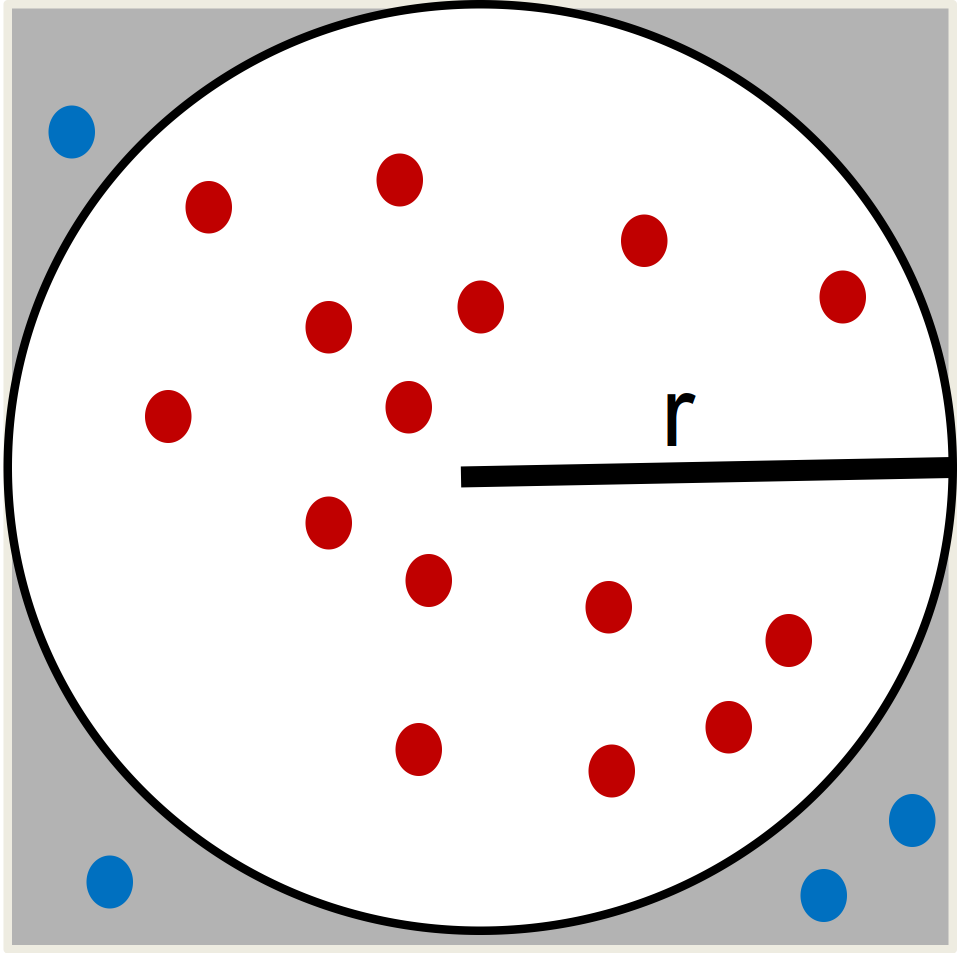
\includegraphics[width=1\textwidth]{pictures/montecarlopi}
	\end{minipage}
\end{example}

\subsection{Diskrete Ereignissimulation}
\subsubsection{Warteschlangentheorie}
Die Warteschlangentheorie beschäftigt sich mit der mathematischen Analyse von Systemen, in denen Aufträge von Bedienungsstationen bearbeitet werden und gibt Antwort auf die Fragen nach den charakteristischen Grössen, wie der Stabilität des Wartesystems, der Anzahl Kunden im System, ihrer Wartezeit etc. Sie unterstützt unter anderem Führungsentscheidungen über den Personaleinsatz und den Abfertigungsprozess. Ihre Anwendung reicht von Telekommunikationssystemen, Verkehrssystemen über Logistik bis zu Fertigungssystemen.
\begin{example}\\
	\begin{tabular}{|l|l|l|}
		\hline
		\textbf{System} & \textbf{Bedienungsstation} & \textbf{Aufträge} \\ \hline
		Bank & Schalter & Kundenbesuche \\ \hline
		Spital & Ärzte, Pflegende, Betten & Patientinnen und Patienten \\ \hline
		Rechner & CPU, I/O-Geräte & Jobs \\ \hline
		Fertigung & Maschinen, Operateure & Bauteile \\ \hline
		Rettungsdienst & Rettungsfahrzeuge, Notfallärzte & Patientinnen und Patienten \\ \hline		
	\end{tabular}
\end{example}

\subsubsection{Hauptmerkmale}
\begin{compactitem}
	\item Anwesenheit stochastischer Prozesse
	\item Zeit(-ablauf) spielt eine wichtige Rolle.
	\item Wertveränderungen der Variablen werden verursacht durch Ereignisse und treten nur an diskreten Zeitpunkten auf.
\end{compactitem}

\begin{multicols}{2}
	\textbf{Vorteile:}
	\begin{compactitem}
		\item Kostengünstiges und sicheres Experimentierfeld
		\item Ermöglicht Analyse komplexer Systeme durch hohen Detaillierungsgrad
		\item Ermöglicht Animation und steigert somit Systemverständnis
	\end{compactitem}
	\textbf{Nachteile:}
	\begin{compactitem}
		\item Erfordert einen hohen initialen Zeitaufwand
		\item Bau eines Simulationsmodells ist relativ fehleranfällig
		\item Interpretation der Analysedaten ist anspruchsvoll
	\end{compactitem} \ \\
\end{multicols}

\subsubsection{M/M/1 Modell}
\begin{multicols}{3}
	\begin{compactitem}[$\bullet$]
		\item M-Elemente betreten Warteschlange
		\item M-Elemente sind in Warteschlange
		\item 1-Element verlässt Warteschlange
	\end{compactitem}
\end{multicols}
\begin{example}\\
	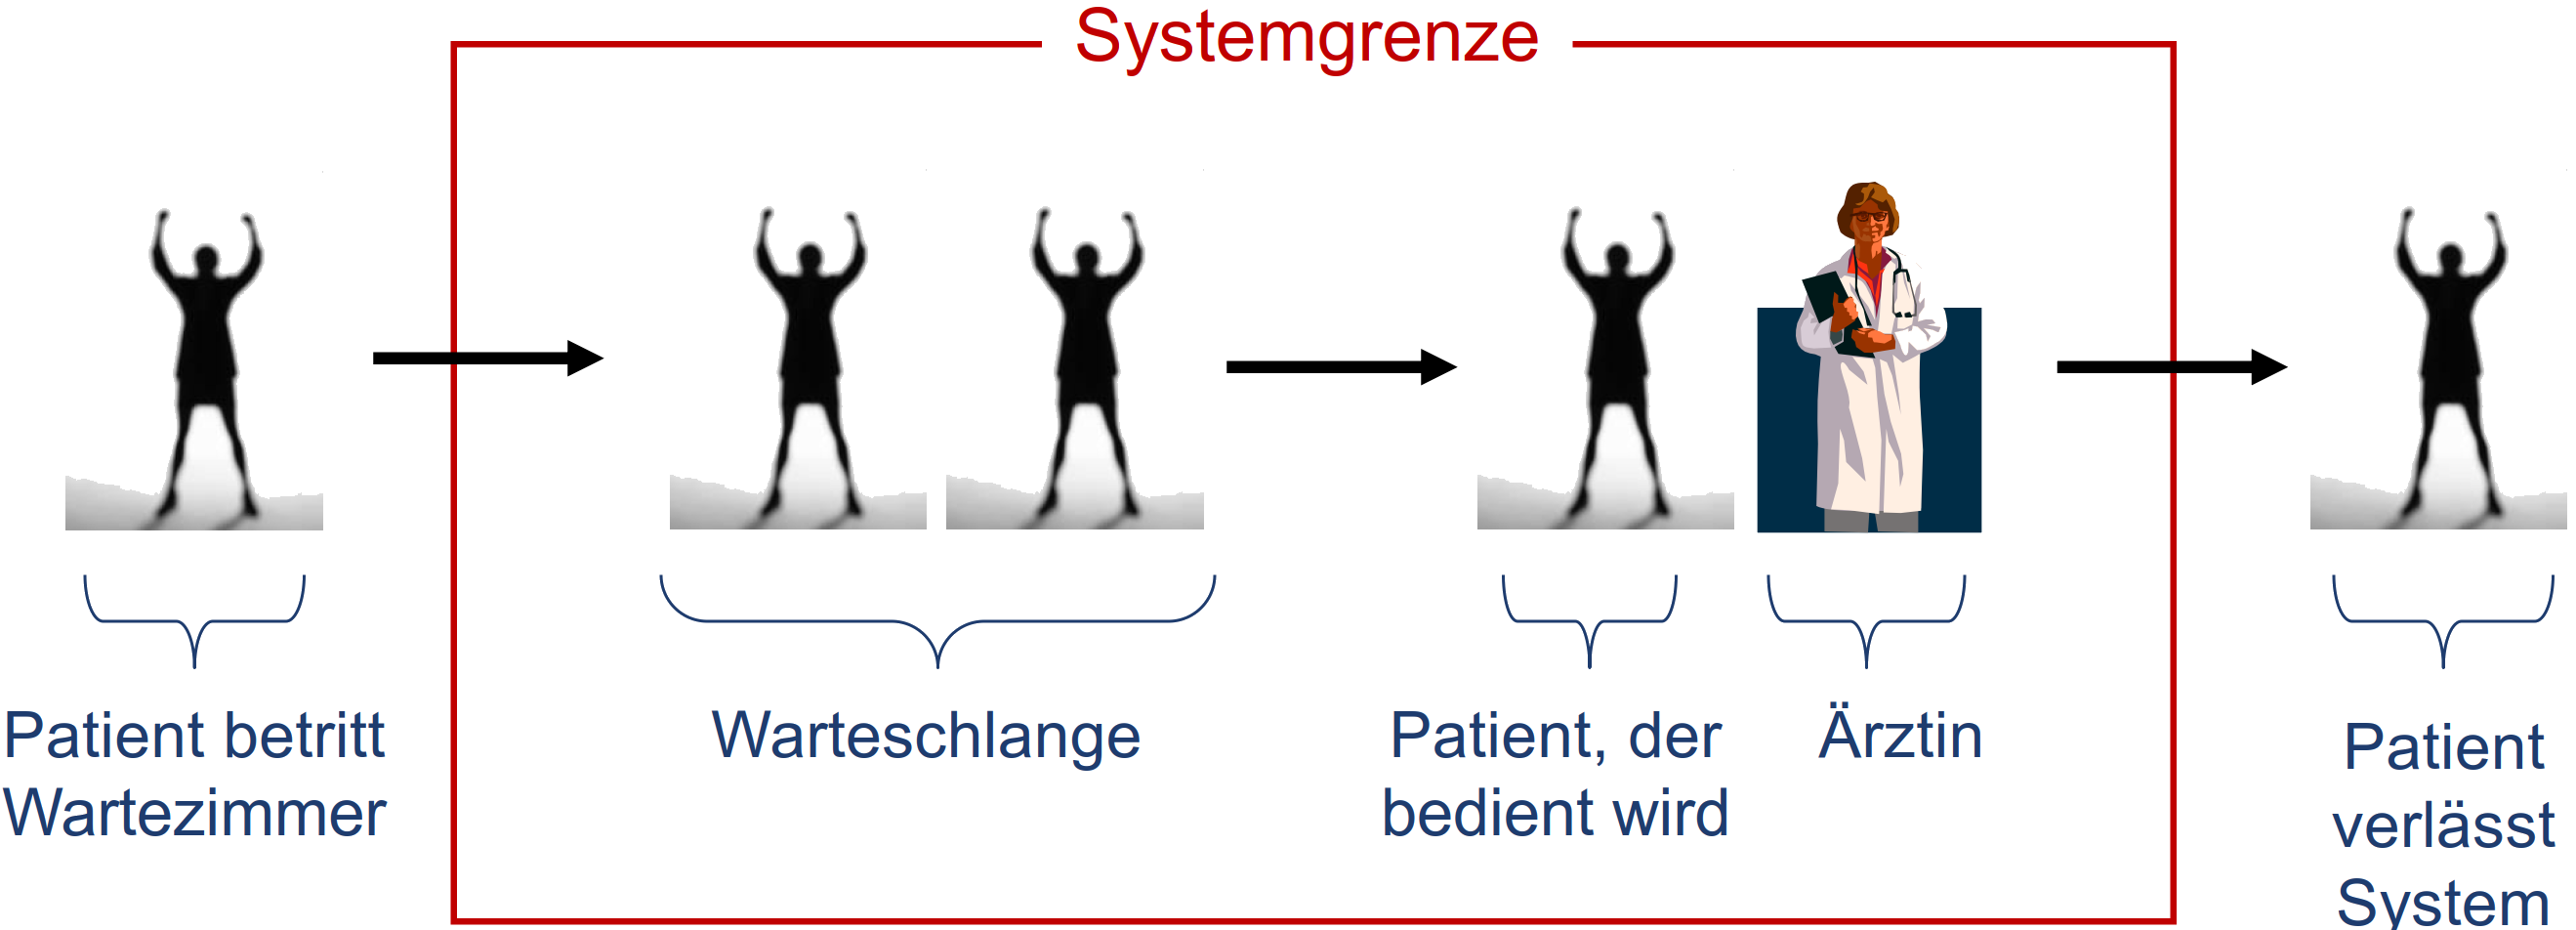
\includegraphics[width=0.7\textwidth]{pictures/mm1modell}
\end{example}
\todo{Folie 32 - Diagramme allenfalls noch einfügen}

\subsubsection{Kernelemente}
\textbf{Items:} Objekte, die durch das System fliessen (z.B. Patienten, Erstzteile, ...). Items haben meistens Attribute (Ankunftszeit, Bearbeitungsstartzeit, Prioritätsklasse, usw.). \\
\textbf{Systemzustand:} Der Zustand $Z(t)$ gibt eine vollständige Beschreibung des Systems am Zeitpunkt $t$. Der Systemzustand ist meistens ein (mehrdimensionaler) Vektor und dient u.a. der Berechnung der Zielgrössen. \\
\textbf{Simulationsuhr:} Die Simulationsuhr hält die virtuelle Zeit im Simulationsmodell fest. \\
\textbf{Ereignis:} Jedes Ereignis hat eine Wirkung, die zum Auftretenszeitpunkt ausgeübt wird. Die Wirkung besteht aus einer Änderung des Systemzustands und/oder einer Änderung der Future-Event-List. In der Zeit zwischen zwei nachfolgenden Ereignissen passiert im System nichts (der Systemzustand ändert sich nicht). Aus diesem Grund kann die Simulationsuhr von Ereignis zu Ereignis springen. \\
\textbf{Future Event List:} Dynamische Liste, die 0 oder mehr (Zeitpunkt-, Ereignis-) Paare enthält; Sie umfasst alle Ereignisse, die zum aktuellen Zeitpunkt bekannt sind. Während eines Simulationslaufs werden ständig neue Ereignisse hinzugefügt und verarbeitete Ereignisse gelöscht.

\subsubsection{Spezifikation eines DE Modells}
DE Modelle werden spezifiziert durch
\begin{compactenum}
	\item Flussdiagramme
	\item Ereignisdiagramme
\end{compactenum}

\begin{example}[Beispiel für nachfolgende Kapitel 4.2.6 - 4.2.7]
	Wir betrachten eine Maschine, worauf genau ein Produkt hergestellt wird. Der Ankunftsprozess der Produktionsaufträge ist poissonverteilt mit dem Parameterwert $\lambda$. Bearbeitungszeiten sind exponentialverteilt mit dem Parameterwert $\mu$.\\
	Bei der Produktion können Fehler auftreten. Beim Maschinenausgang werden die Produkte visuell kontrolliert. Die Wahrscheinlichkeit eines Fehlers ist $\epsilon$. Misslungene Produktionsaufträge müssen wiederholt werden. \\
	\textbf{Items:} Produktionsaufträge mit Attributen: Ankunftszeit, Bearbeitungsstartzeit, Bearbeitungszeit, Anzahl Fehlversuche, etc. \\
	\textbf{Zustand:} $Z$ = (Anzahl) Produktionsaufträge im System \\
	\textbf{Ereignisse:} $e_1$ = Ankunft eines Produktionsauftrags; $e_2$ = Bearbeitung auf der Maschine abgeschlossen
\end{example}

\subsubsection{Flussdiagramm}
\textbf{Grundbausteine:}
\begin{multicols}{5}
	Quelle und Senke: \\ \\
	Fluss: \\ \\
	Weiche: \\ \\
	Warteschlange: \\ \\
	Aktivität oder Ressource:
\end{multicols}	
\begin{multicols}{5}
	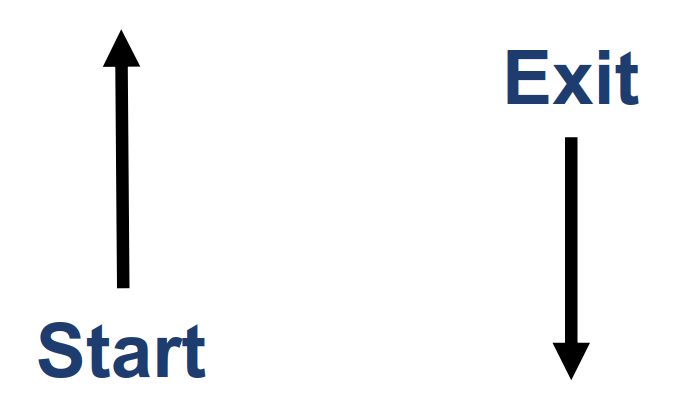
\includegraphics[width=0.15\textwidth]{pictures/fluss_quelle_senke}\\ \\
	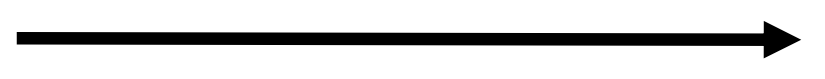
\includegraphics[width=0.15\textwidth]{pictures/fluss_fluss}\\
	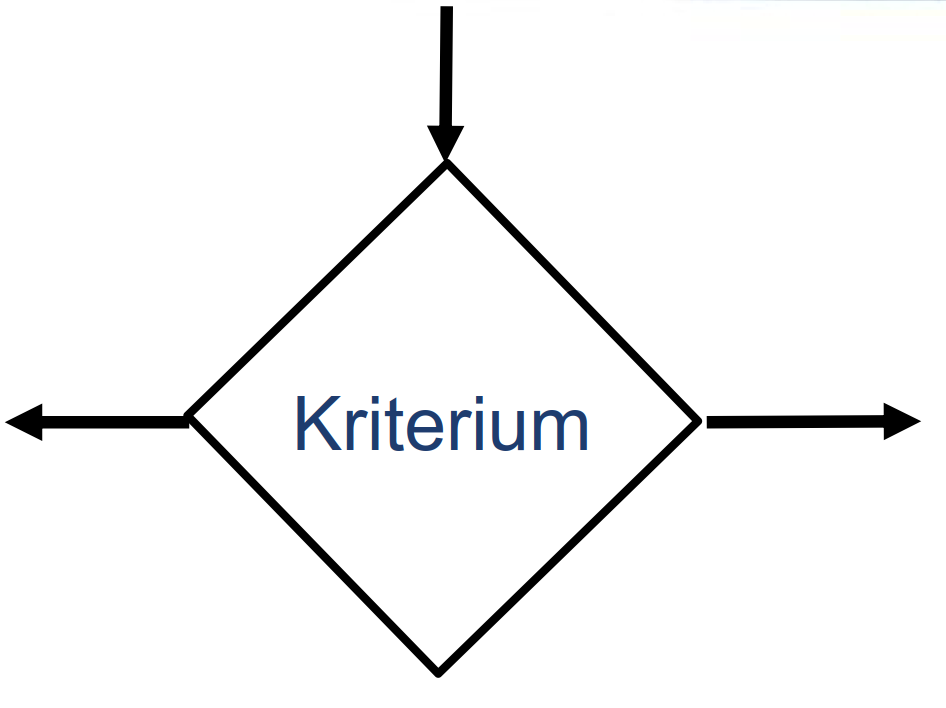
\includegraphics[width=0.15\textwidth]{pictures/fluss_weiche}\\ 
	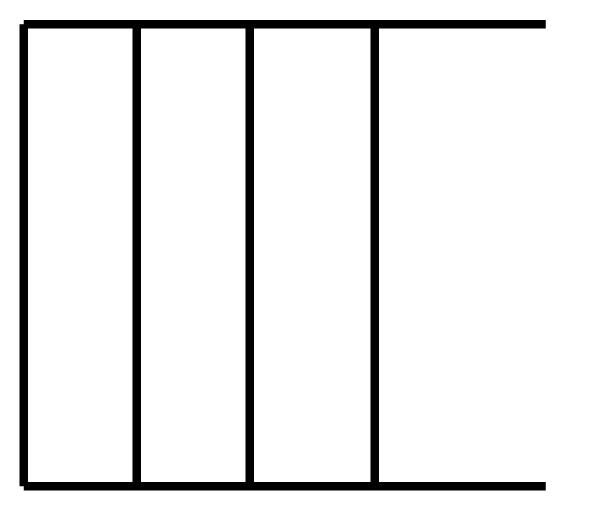
\includegraphics[width=0.1\textwidth]{pictures/fluss_warteschlange}\\ 
	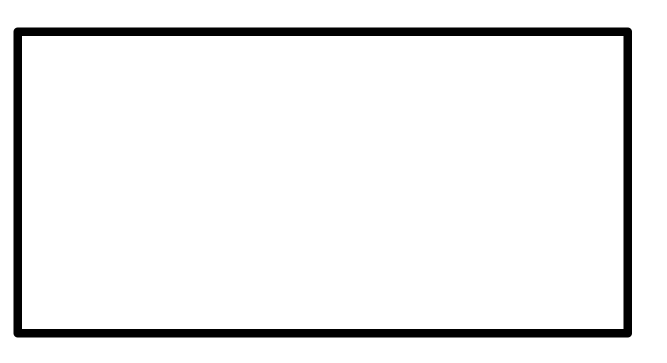
\includegraphics[width=0.15\textwidth]{pictures/fluss_aktivitaet}
\end{multicols}
\begin{multicols}{2}
	\begin{multicols}{2}
		Gabelung (konvergent):\\
		Gabelung (divergent):
	\end{multicols}
	Lager:
\end{multicols}
\begin{multicols}{2}
	\begin{multicols}{2}
		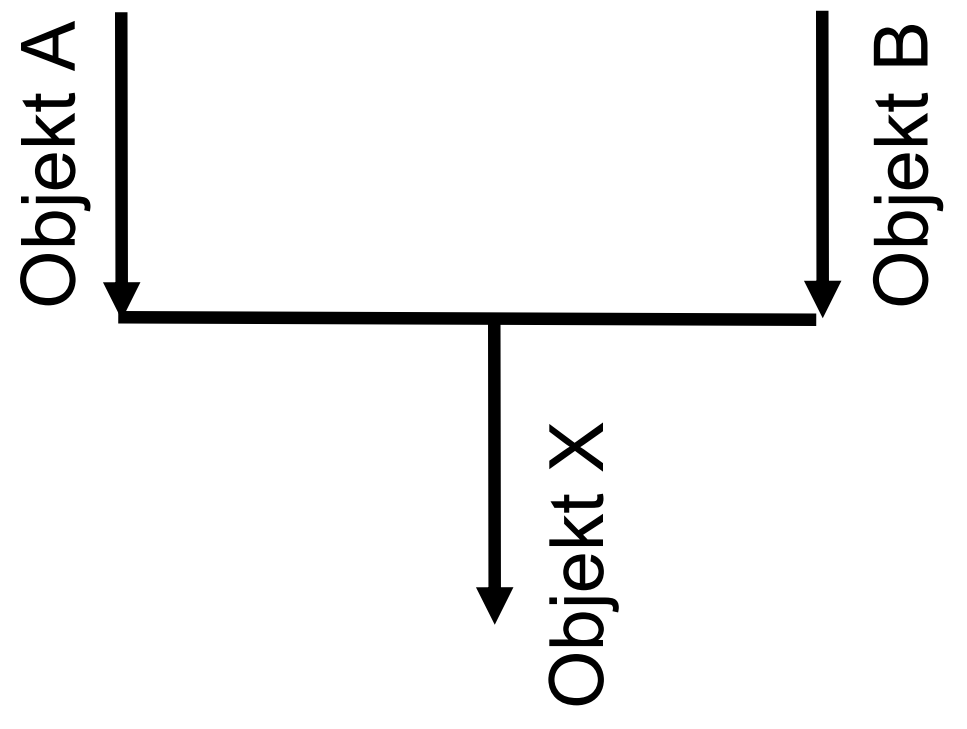
\includegraphics[width=0.2\textwidth]{pictures/fluss_gabelung1}\\ 
		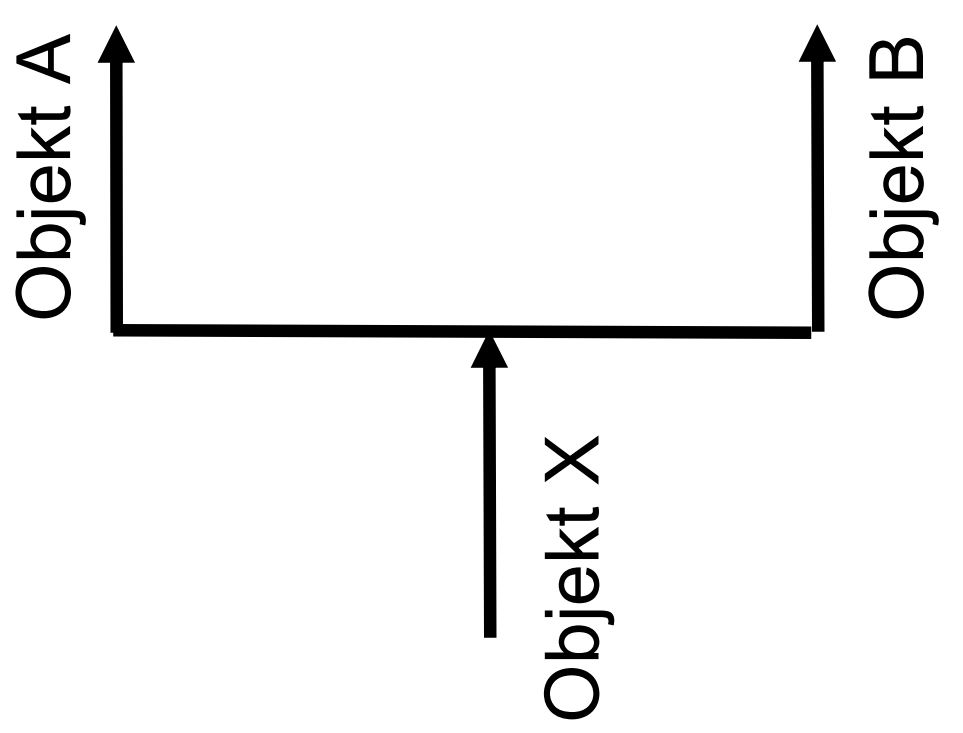
\includegraphics[width=0.2\textwidth]{pictures/fluss_gabelung2}
	\end{multicols}
	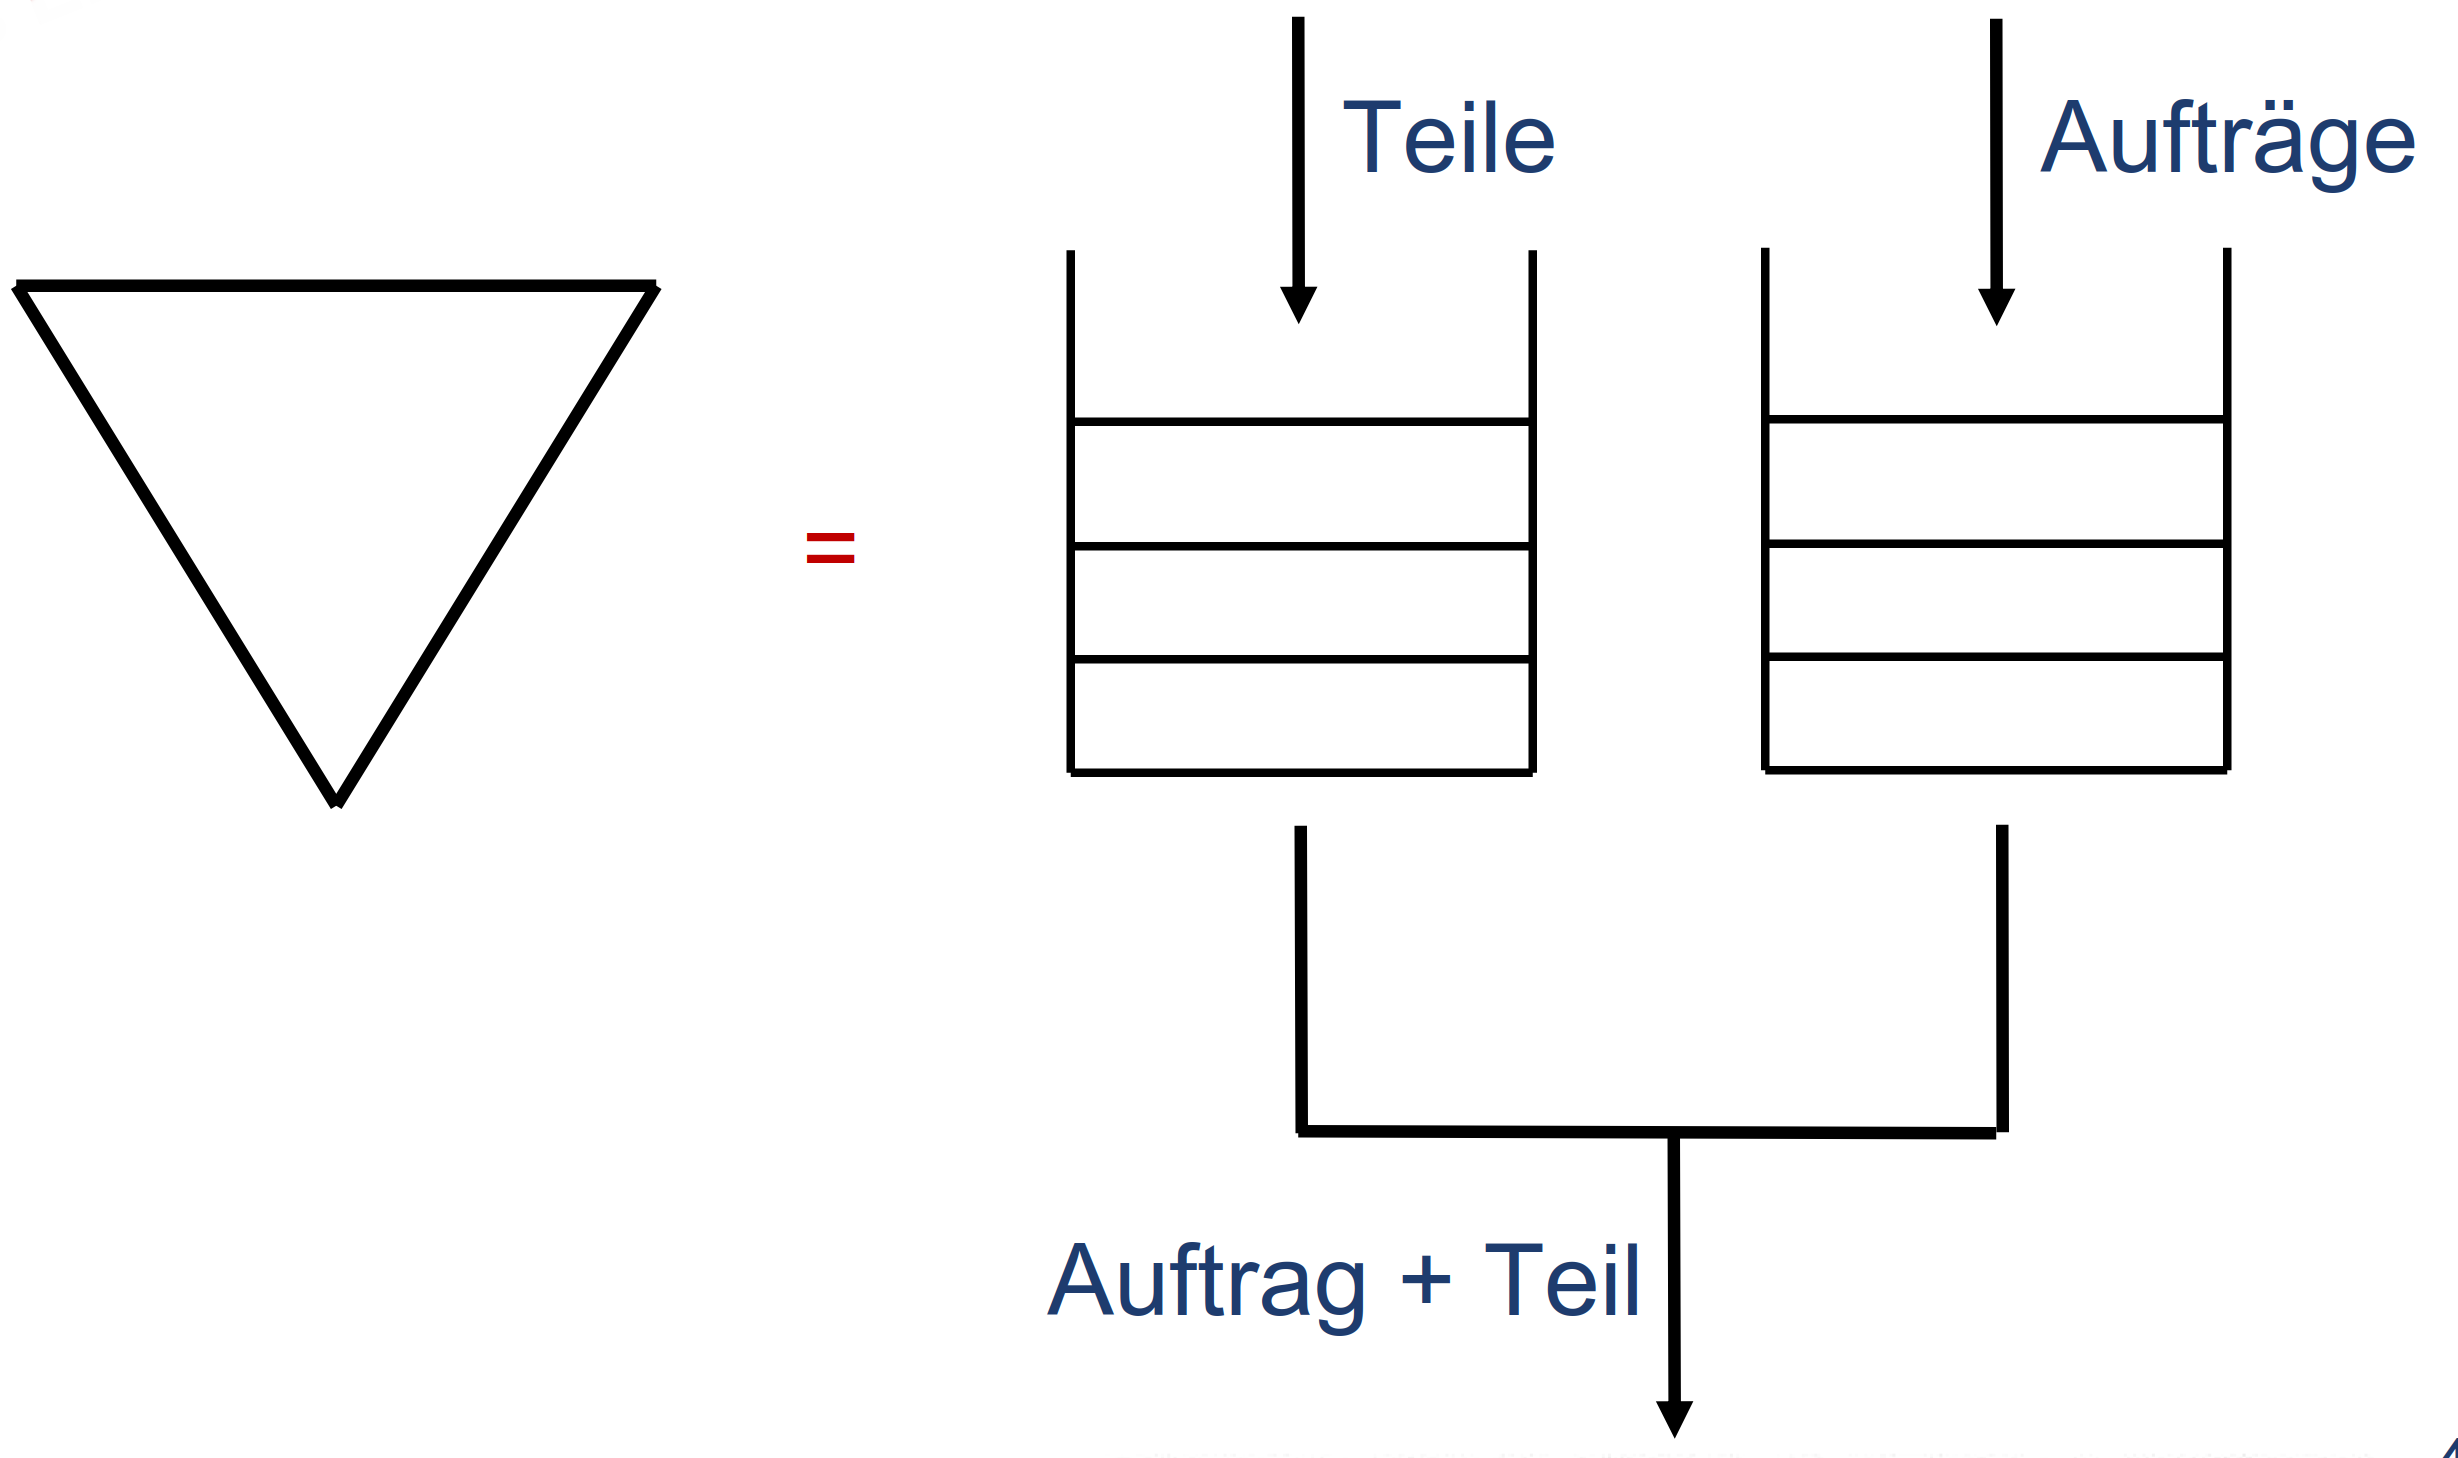
\includegraphics[width=0.4\textwidth]{pictures/fluss_lager}
\end{multicols}
\begin{example} \\
	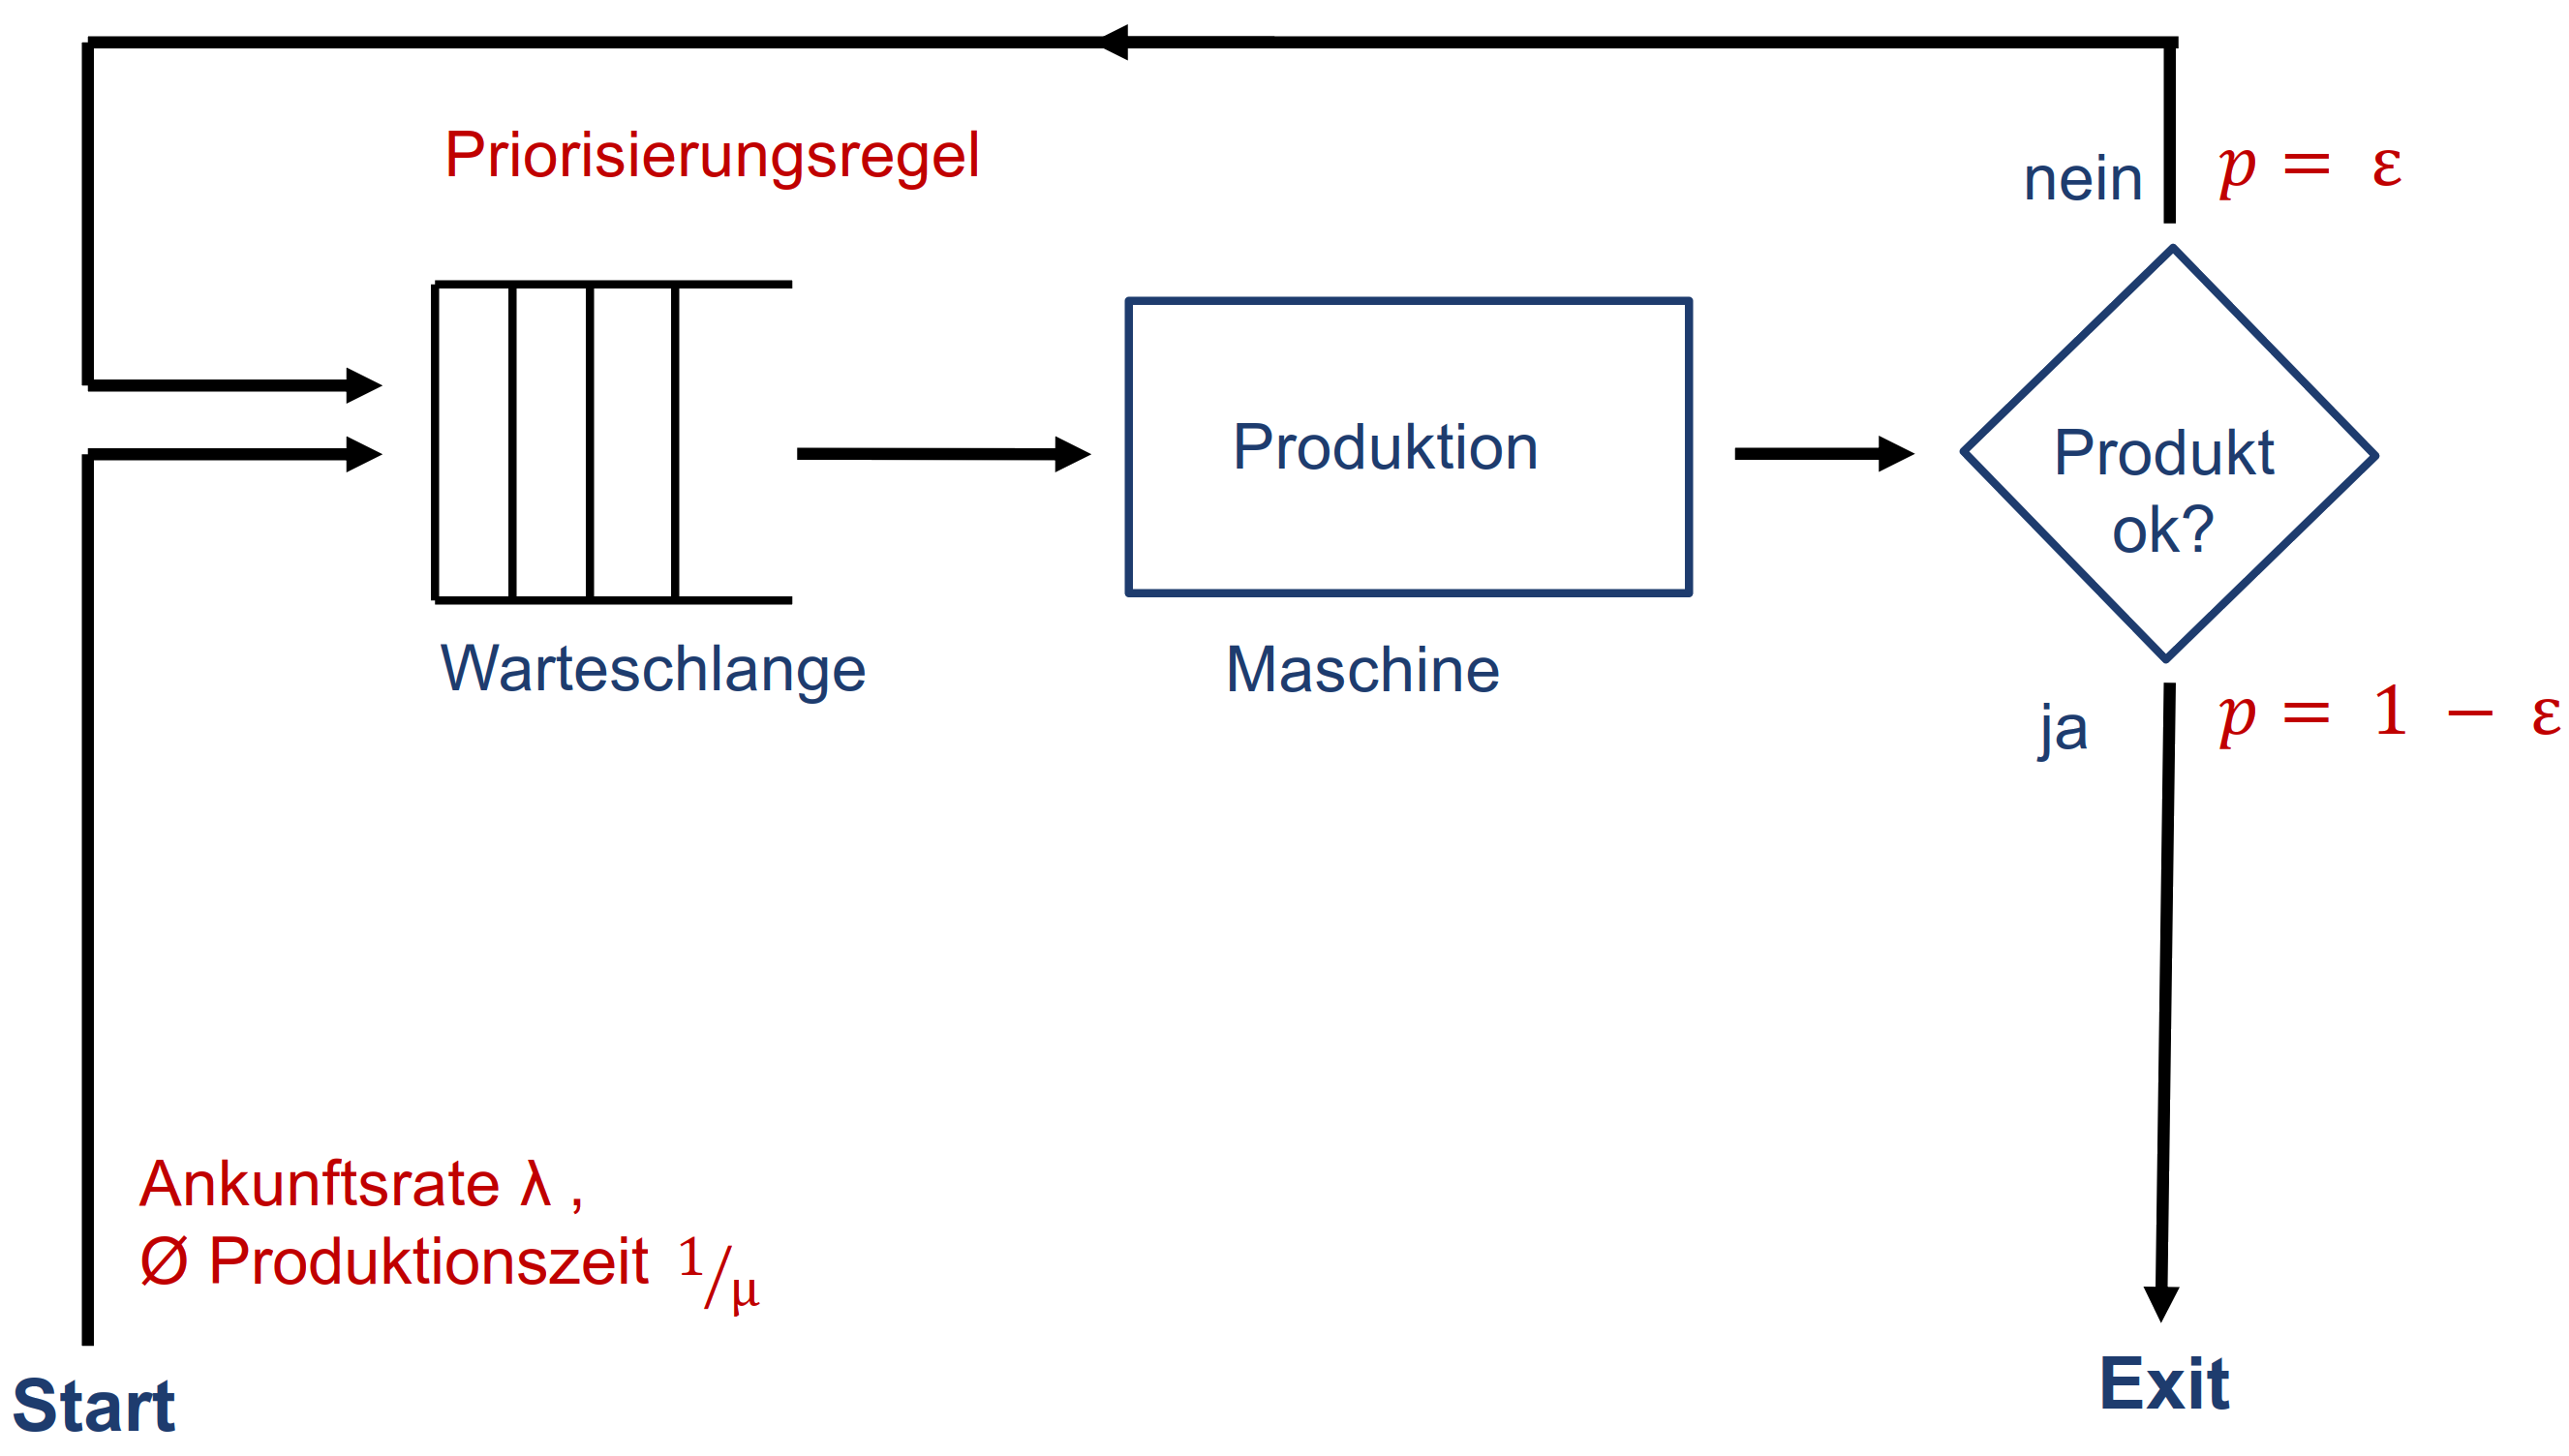
\includegraphics[width=0.5\textwidth]{pictures/flussdiagramm}
\end{example}

\subsubsection{Ereignisdiagramm}
\begin{example} 
	\begin{multicols}{2}
		\textbf{Ereignisdiagramm $e_1$:} \\
		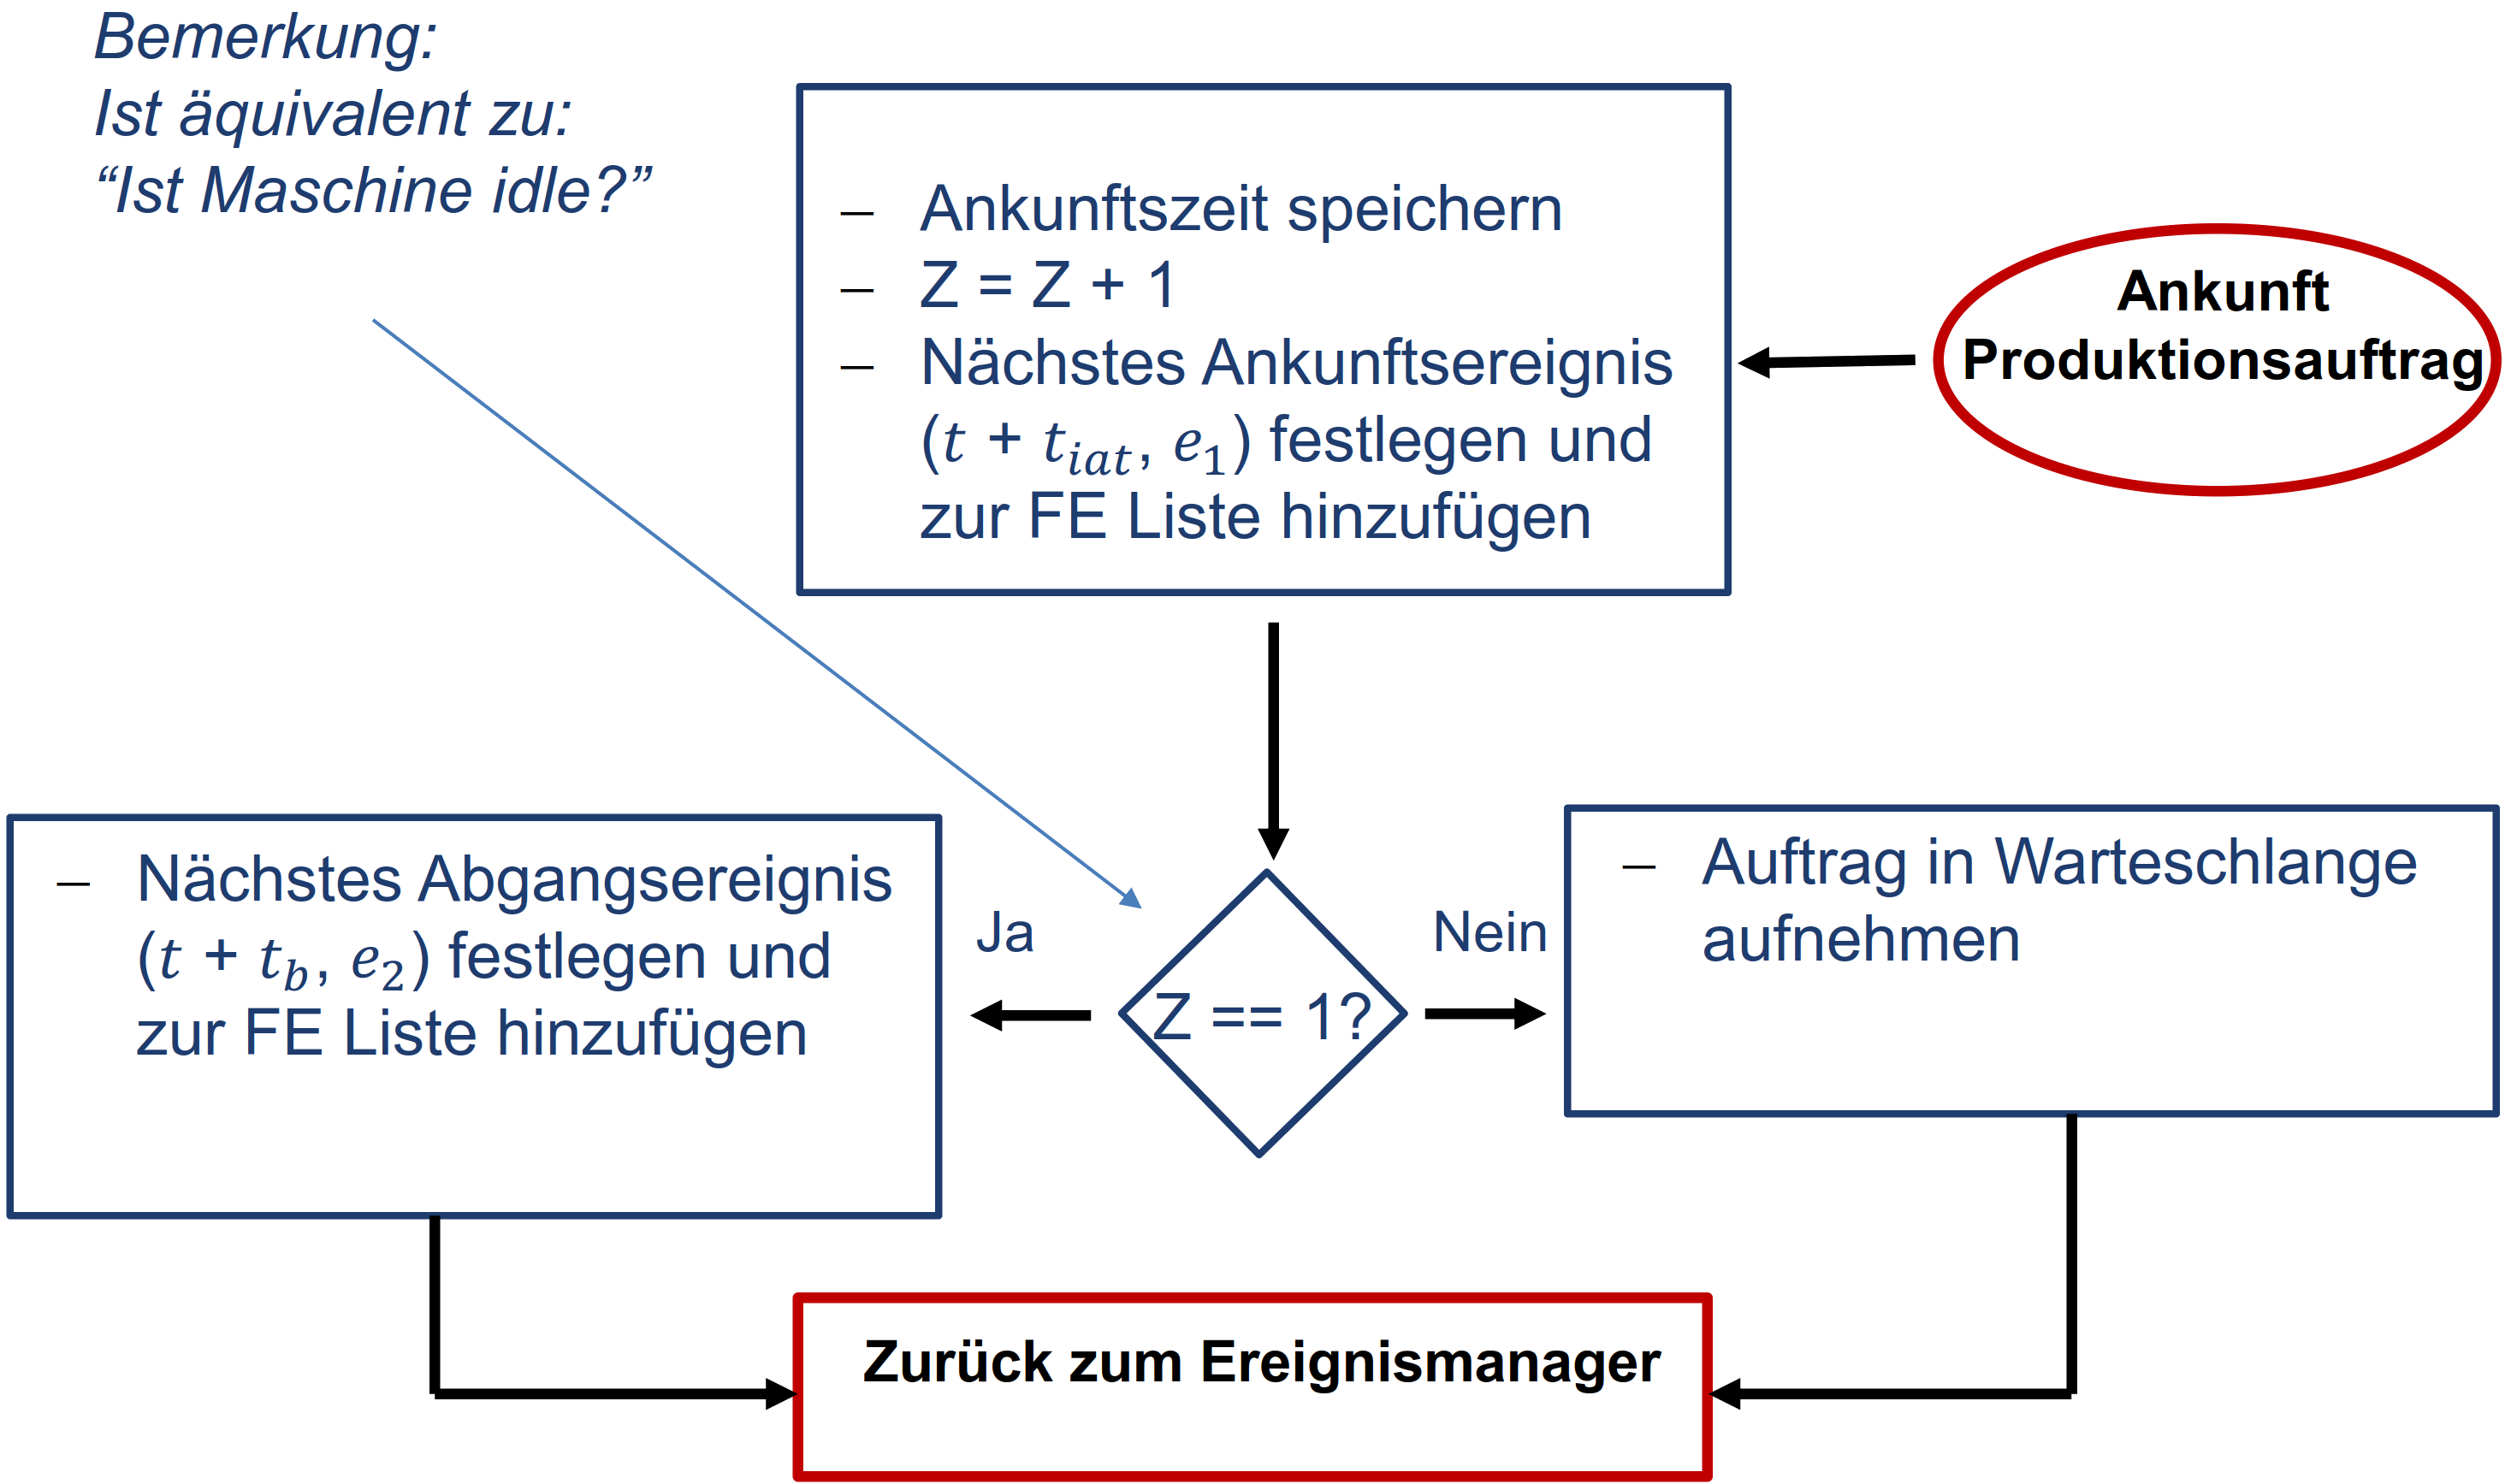
\includegraphics[width=0.5\textwidth]{pictures/ereignisdiagramm1}
		\textbf{Ereignisdiagramm $e_2$:} \\
		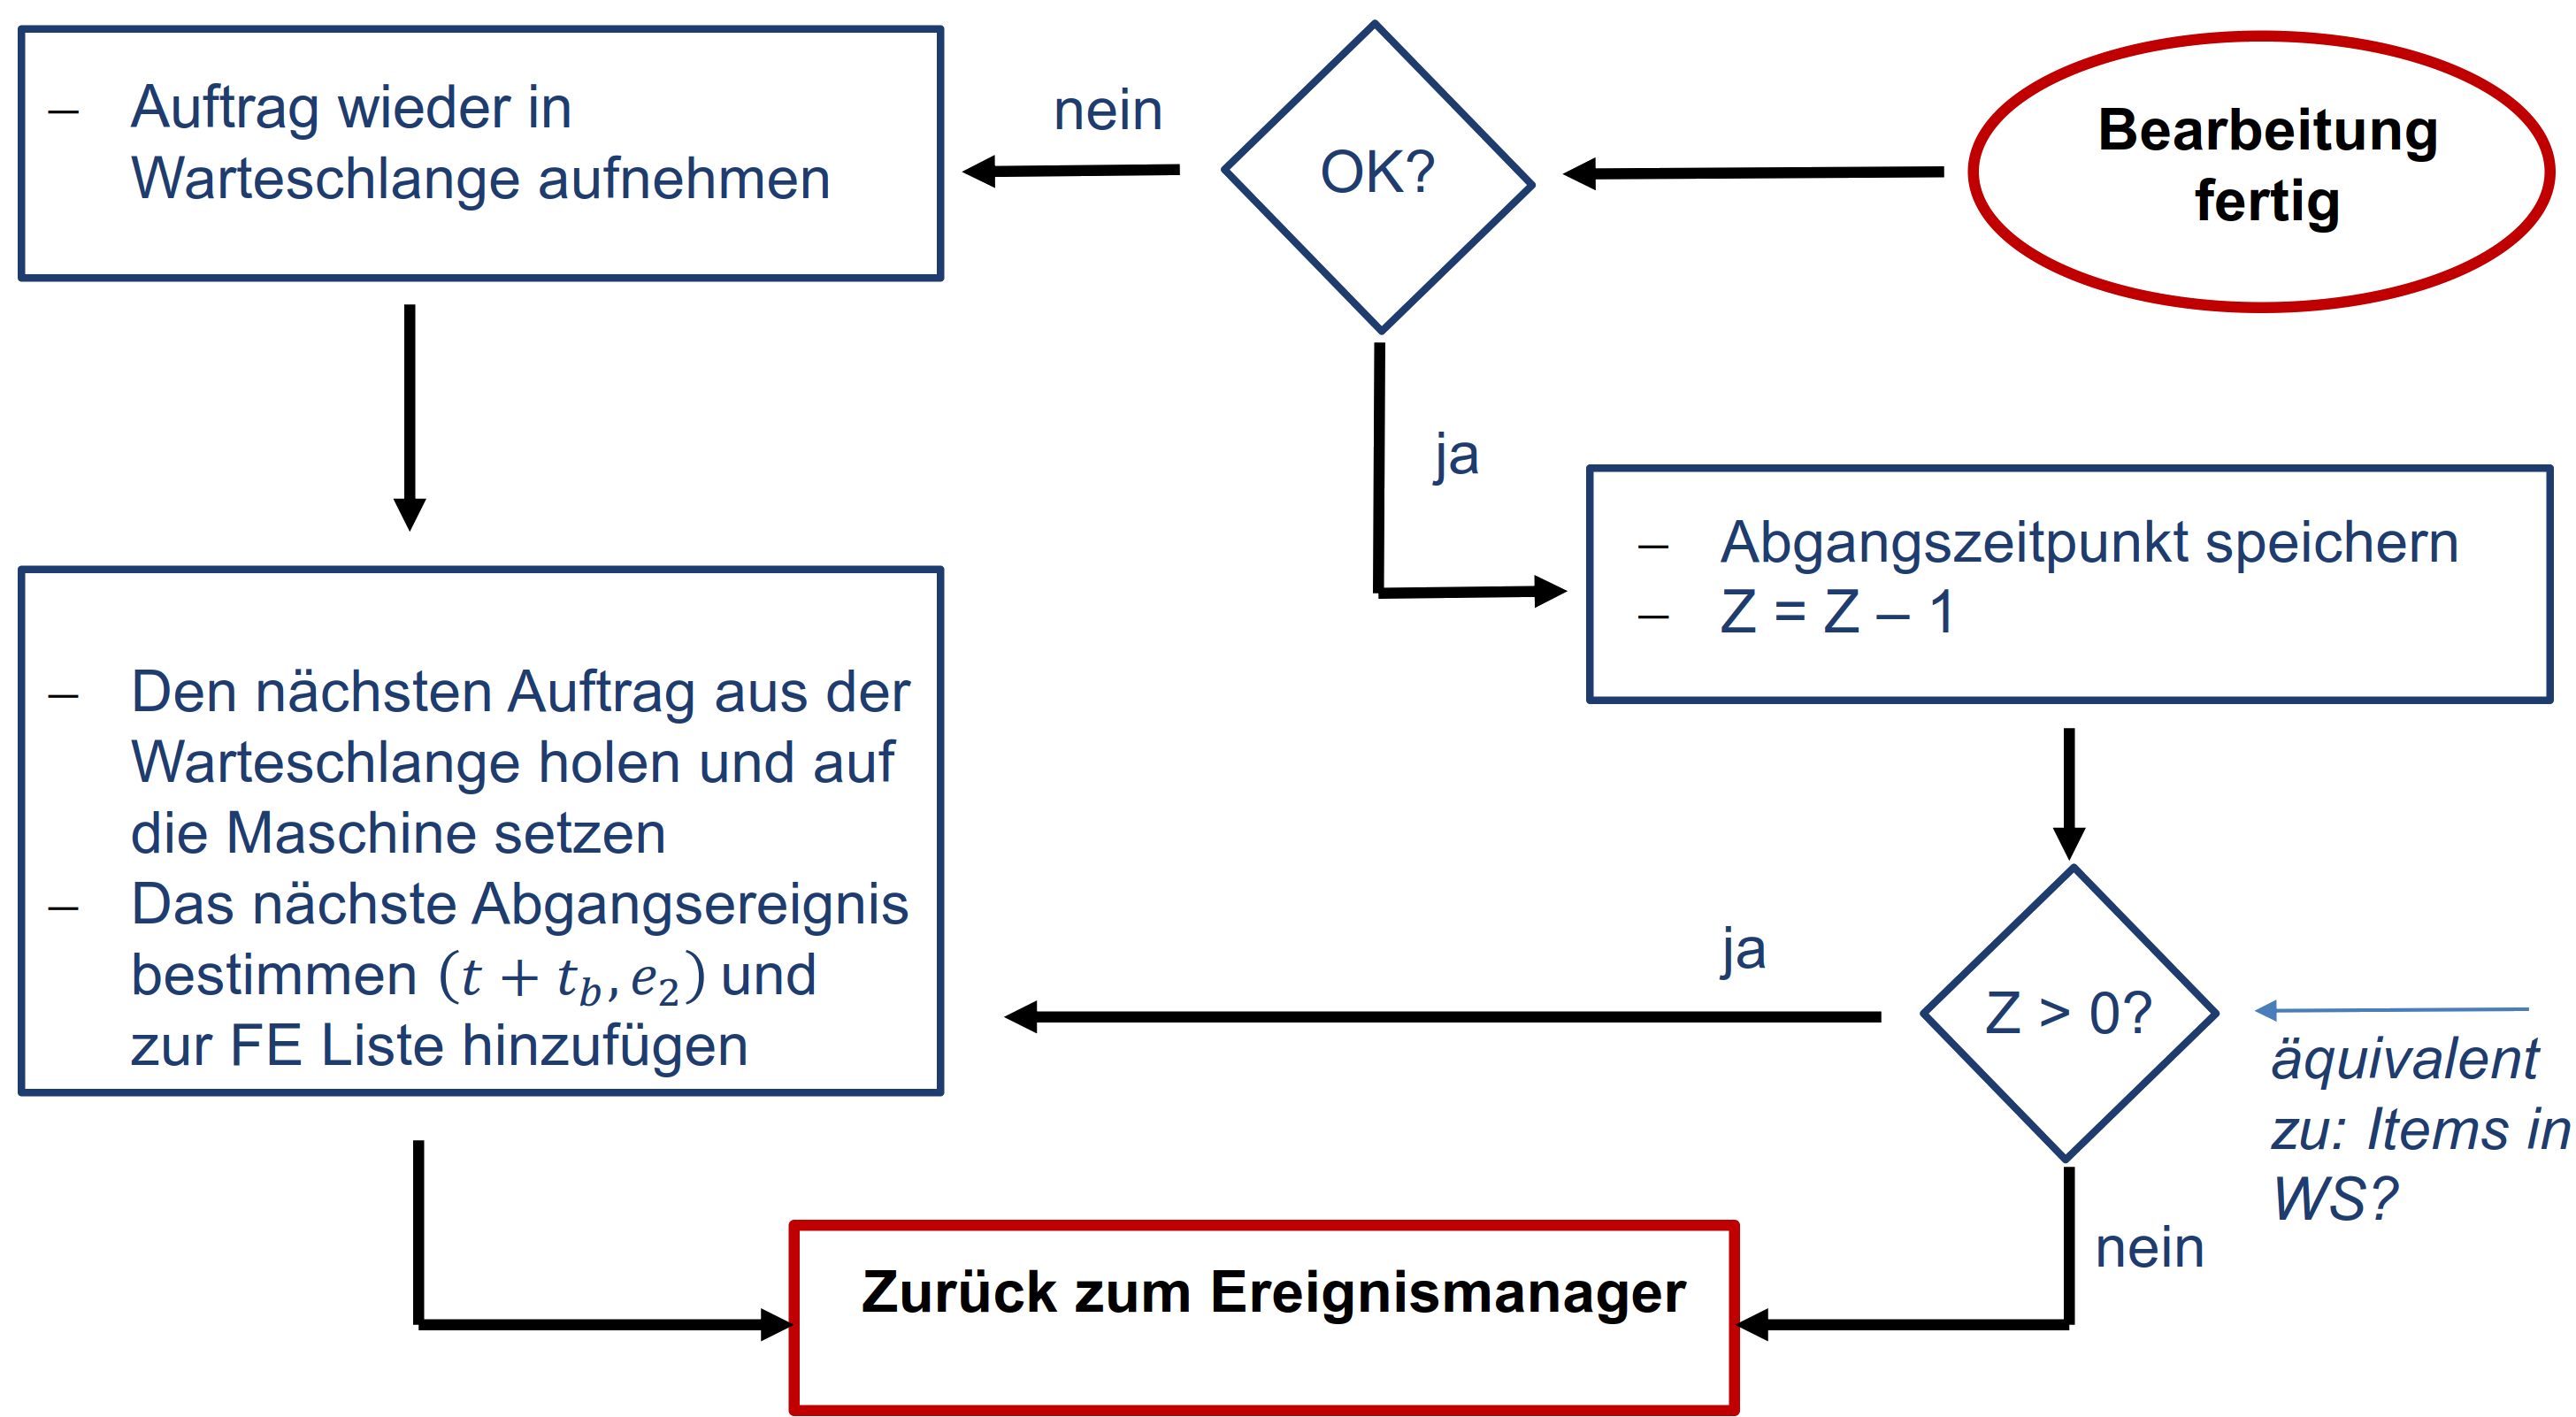
\includegraphics[width=0.5\textwidth]{pictures/ereignisdiagramm2}
	\end{multicols}
\end{example}

\subsubsection{Simulationskern / Ereignismanager}
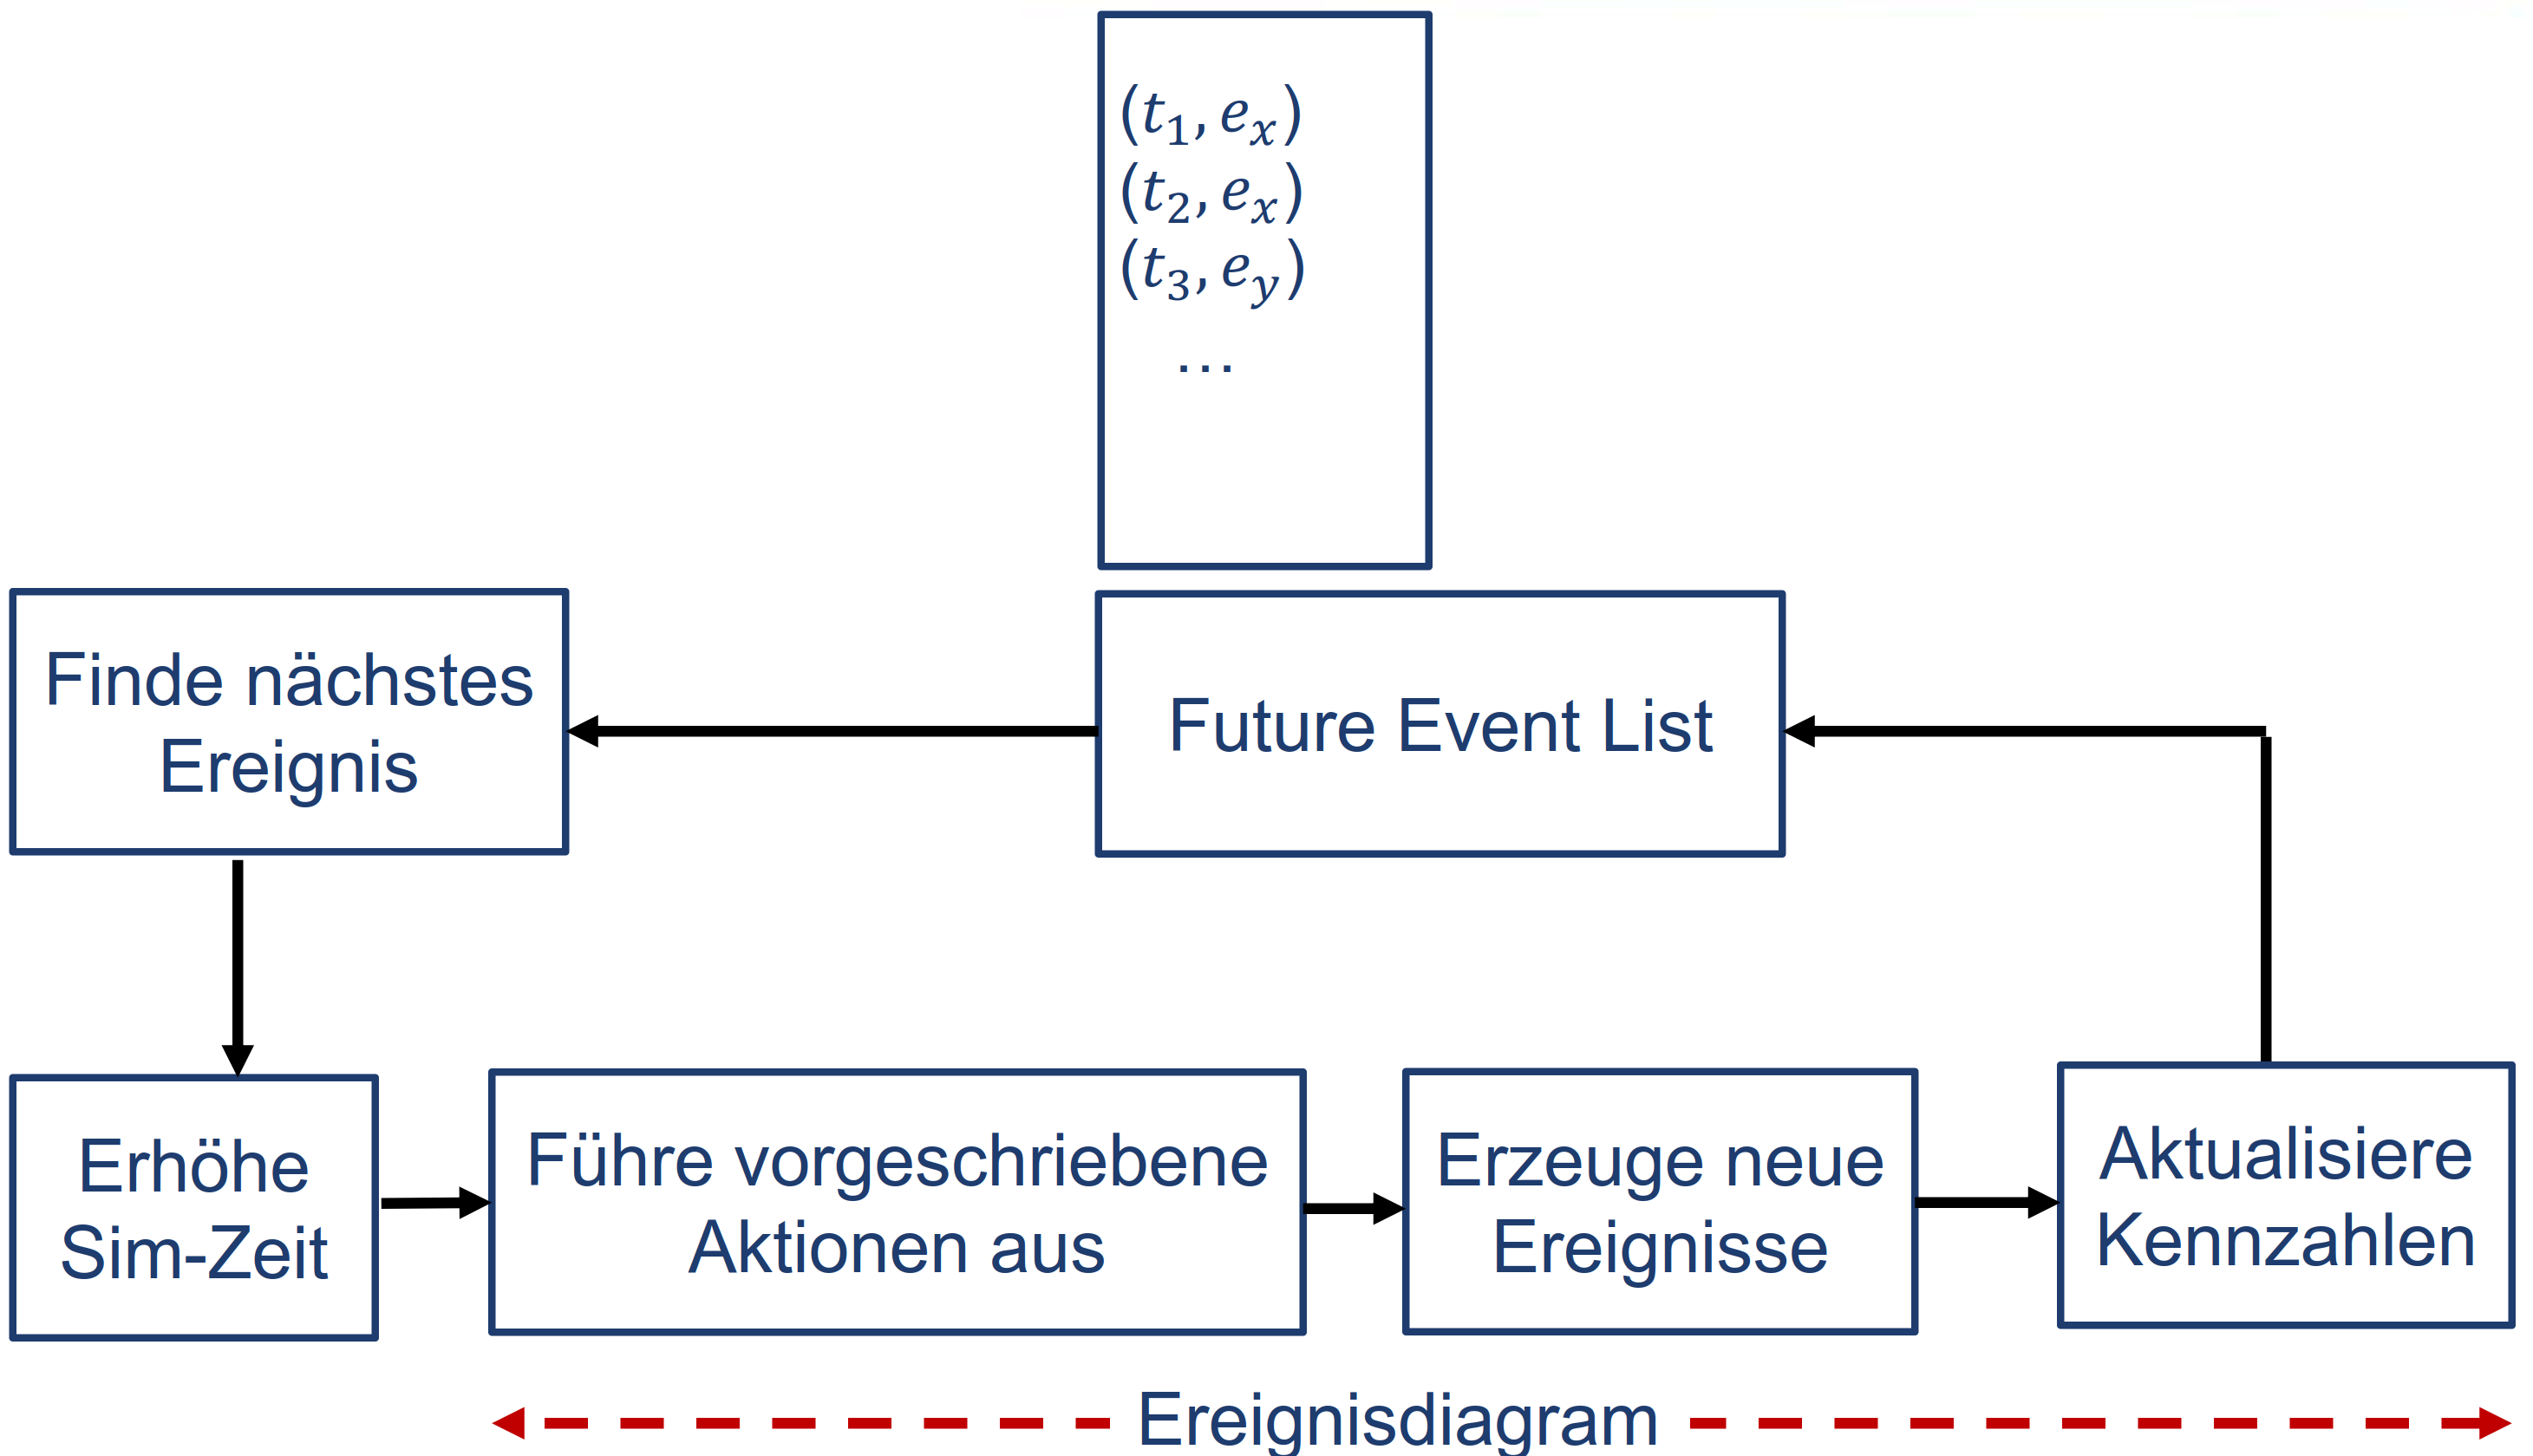
\includegraphics[width=0.5\textwidth]{pictures/ereignismanager}

\subsection{Wahrscheinlichkeitsverteilungen}	
\textbf{Vorteile:} 	
\begin{compactitem}
	\item Kompakte Formulierung (meistens 1 oder 2 Parameter)
	\item Leicht anzupassen (über die geringe Anzahl Parameter)
	\item Grosser Bereich an ausgewürfelten Zufallszahlen
\end{compactitem}	
\textbf{Nachteile:}
\begin{compactitem}
	\item Beschränkte Anzahl Parameter, um die Verteilung in die gewünschte Richtung anzupassen. Manchmal einfach nicht möglich, die komplexe Wirklichkeit in einer Verteilung mit 1 oder 2 Parametern abzubilden.
	\item Verteilung repräsentiert die Wirklichkeit oft nicht gut in Extremsituationen.
\end{compactitem}

\begin{multicols}{3}
	\subsubsection{Uniformverteilung} 
	$X \sim U[0, 200]$ \\
	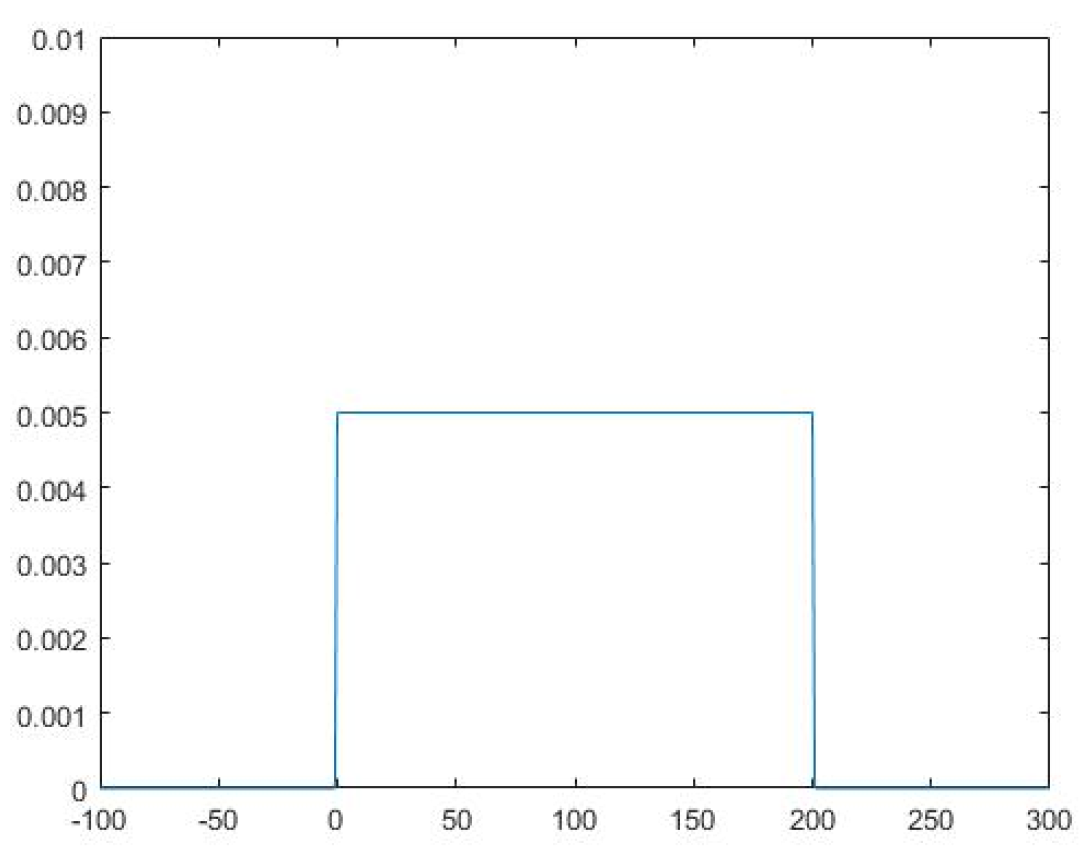
\includegraphics[width=0.25\textwidth]{pictures/uniformverteilung} 
	\subsubsection{Normalverteilung} 
	$X \sim N(100, 10'000)$ \\
	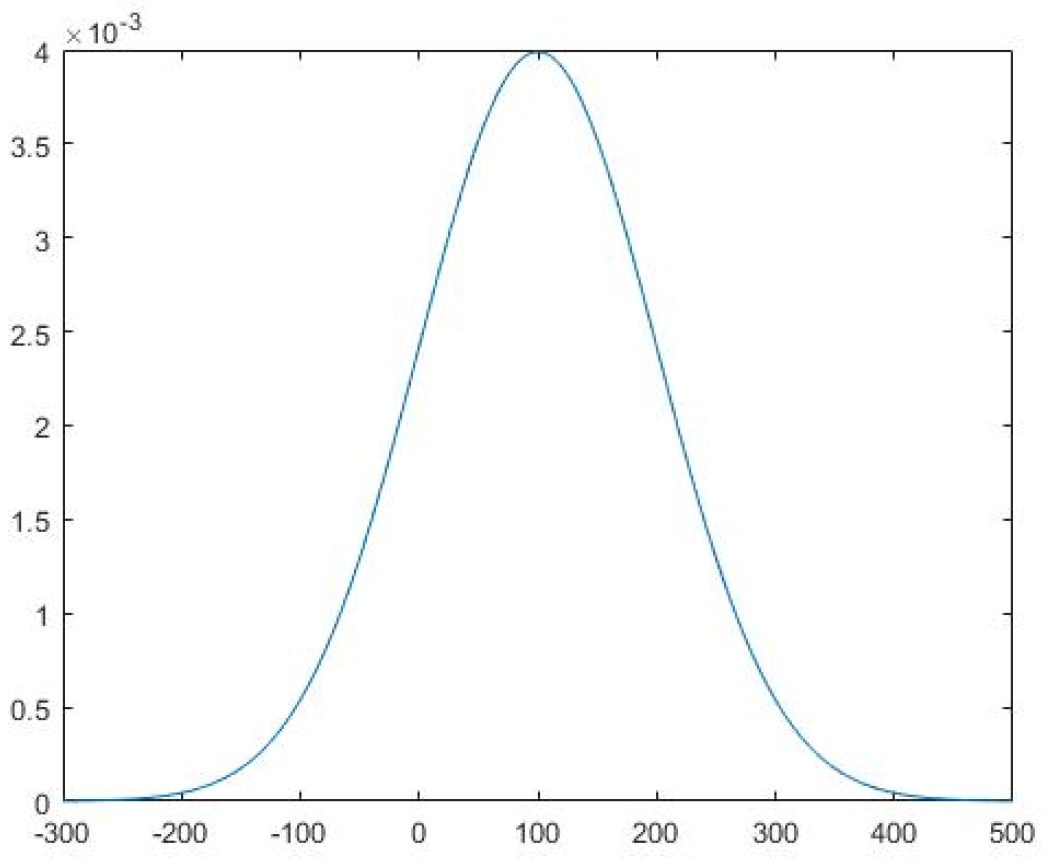
\includegraphics[width=0.25\textwidth]{pictures/normalverteilung} 
	\subsubsection{Poissonverteilung}
	$X \sim P(4)$ \\
	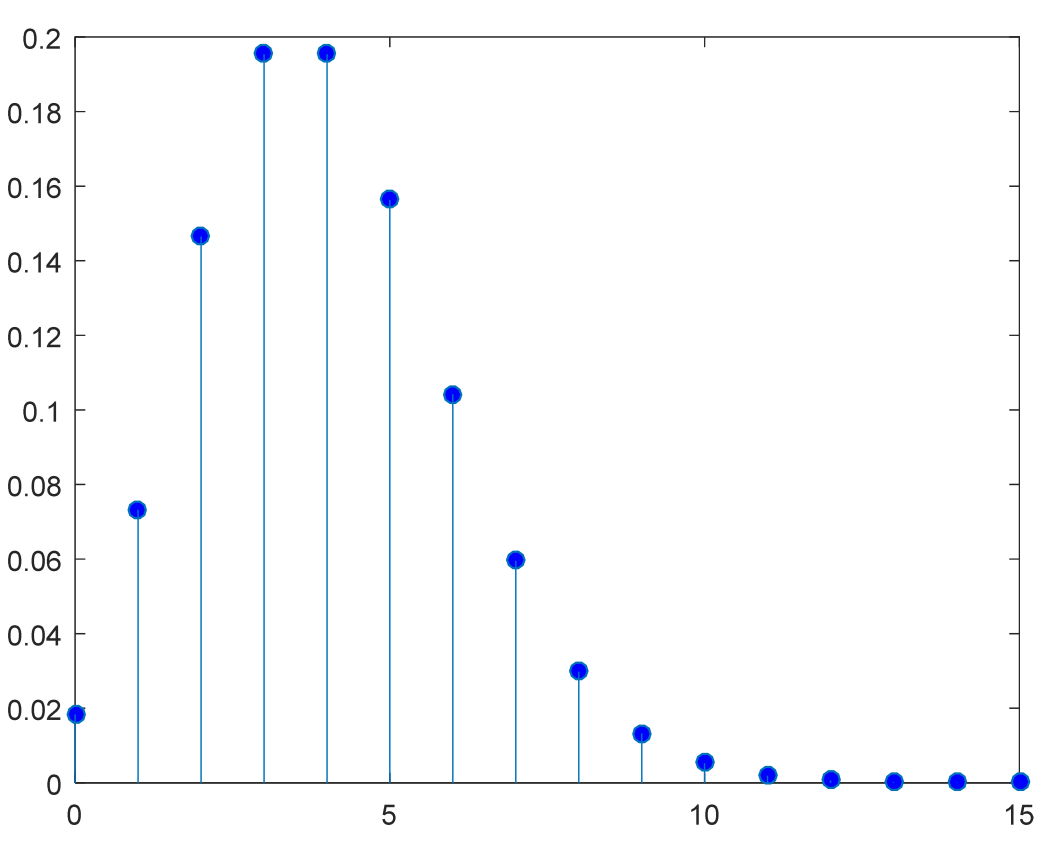
\includegraphics[width=0.25\textwidth]{pictures/poissonverteilung} 
\end{multicols}

\subsubsection{Empirische Verteilung}
\begin{multicols}{2}
	\begin{tabular}{|l|l|}
		\hline
		\textbf{Zufallszahl} & \textbf{Wahrscheinlichkeit} \\ \hline
		1 & 0.4 \\ \hline
		2 & 0.3 \\ \hline
		4 & 0.1 \\ \hline
		8 & 0.15 \\ \hline
		16 & 0.05 \\ \hline
	\end{tabular} \\
	\textbf{Vorteile:}
	\begin{compactitem}
		\item Basiert auf realen Daten
		\item Alle möglichen Formen sind möglich
	\end{compactitem}	
	\textbf{Nachteile:}
	\begin{compactitem}
		\item Es können keine Zufallszahlen erzeugt werden, die nicht schon in der Vergangenheit aufgetreten sind. Daher braucht man eine lange	Historie.
		\item Empirische Verteilungen kann man nicht kompakt auf Papier darstellen.
	\end{compactitem}
\end{multicols}

\subsubsection{Parameterschätzungen Gefahren}
\begin{multicols}{2}
	\begin{compactitem}
		\item Zu wenig Datenmaterial
		\item Nicht-repräsentative Vergangenheitsdaten
		\item Unberücksichtigte Ausreisser
		\item Unerkannte Zeitmuster (Sommer / Winter, Mo-Fr versus Sa-So)
		\item Falsche Interpretation des vorhandenen Datenmaterials
	\end{compactitem}
\end{multicols}

\subsection{Zufallszahlen}
\textbf{Grobe Definition:} Eine Bit-Reihenfolge ist willkürlich, wenn sie auf keine Weise ein Muster enthält. \\
\textbf{Zufallszahlengenerator:} Erzeugt Zufallszahlen zwischen 0 und 1 (und wandelt sie bei Bedarf in Zufallszahlen aus der gewünschten Wahrscheinlichkeitsverteilung um). \\ \\
\textbf{Anforderungen:}
\begin{multicols}{2}
	\begin{compactitem}
		\item Unabhängigkeit (auch die Elemente jeder Teilfolge)
		\item Gleichverteilung (empirische Verteilung weitgehend konstant)
		\item Besetzungsdichte (keine Lücken)
		\item Keine Periodizität
		\item Schneller und speichereffizienter Generator
		\item allenfalls Reproduzierbarkeit
	\end{compactitem}
\end{multicols}	
\textbf{Bemerkung:} Wirkliche Zufallszahlen sind nicht reproduzierbar. In den meisten Fällen will man die Zufallszahlen aber reproduzieren können. Wir sprechen in dem Fall von Pseudo – Zufallszahlen.
	
\subsubsection{Deterministische Reihenfolge}
\begin{compactitem}
	\item Jede Zufallszahl wird direkt aus ihrem unmittelbaren Vorgänger erzeugt.
	\item Die Erzeugung von Zufallszahlen startet mit einem initialen Wert. Dieser erste Wert des Zahlenflusses wird als Seed bezeichnet.
	\item Der Seedwert legt den gesamten Zahlenfluss eindeutig fest. D.h., wenn die Seedwerte identisch sind, sind die Zahlenflüsse, die sie auslösen, es auch.
\end{compactitem}

\subsubsection{Lineare Kongruenzmethode}
\textbf{Formel:} $X_{i+1}=(aX_i+c)\mod m$ mit $a$, $c$, $m$ und $X_0$ als Integer und $m > 0$, $a < m$, $c < m$ und $X_0 < m$ \\
somit gilt: $u_i = \frac{X_i}{m-1}\sim U(0, 1)$ \\
Die Qualität des Zufallszahlengenerators hängt stark von a, c und m ab. Die wichtigsten Parameter sind a und m; Meistens wählt man sehr hohe (Prim-)Zahlen. \\
\textbf{Problem:} In den allermeisten Fällen brauchen wir keine uniformverteile Zufallszahlen zwischen 0 und 1 sondern Zufallszahlen die aus einer anderen Verteilung stammen.

\subsubsection{Intervallmethode (Diskrete Zielverteilung)}
\begin{minipage}[h]{0.6\textwidth}
	\begin{tabular}{|l|l|l|l|}
		\hline
		\textbf{i} & \textbf{Zufallszahl}($r_i$) & \textbf{Wahrscheinlichkeit} & \textbf{Intervall} ($c_{i-1}$, $c_i$) \\ \hline
		1 & 1 & 0.4 & [0.00, 0.4) \\ \hline
		2 & 2 & 0.3 & [0.40, 0.7) \\ \hline
		3 & 4 & 0.15 & [0.70, 0.85) \\ \hline
		4 & 5 & 0.1 & [0.85, 0.95) \\ \hline
		5 & 18 & 0.05 & [0.95, 1.0) \\ \hline
	\end{tabular}
\end{minipage}
\begin{minipage}[h]{0.3\textwidth}
	\begin{lstlisting}[mathescape=true, tabsize=2]
x= U(0,1); // Standard Zufallszahl 
           // zwischen 0 und 1
for i = 1 : n
	if $c_{i-1}$ =< x < $c_i$
		returnValue = $r_i$;
		break;
	end
end
	\end{lstlisting}
\end{minipage}

\subsubsection{Inversionsmethode (Kontinuierliche Zielverteilung)}
\begin{compactenum}
	\item Generiere $x\sim U(0, 1)$
	\item Berechne $y = F_y^{-1}(x)$ 
\end{compactenum}
\begin{example}
	Uniformverteilung im Bereich [a, b] 
	\begin{multicols}{2}
		\begin{compactitem}
			\item Gegeben: $x\sim U(0, 1)$
			\item Gesucht: $y\sim U(a, b)$
			\item Transformation: $y = a+(b-a)x$
			\item Beachte: $F_y(y) = \left\{\begin{array}{ll}
												0 & y < 0 \\
												\frac{y-a}{b-a} & a \leq y < b \\
												1 & y \geq b \\
											\end{array}\right.$
		\end{compactitem}
		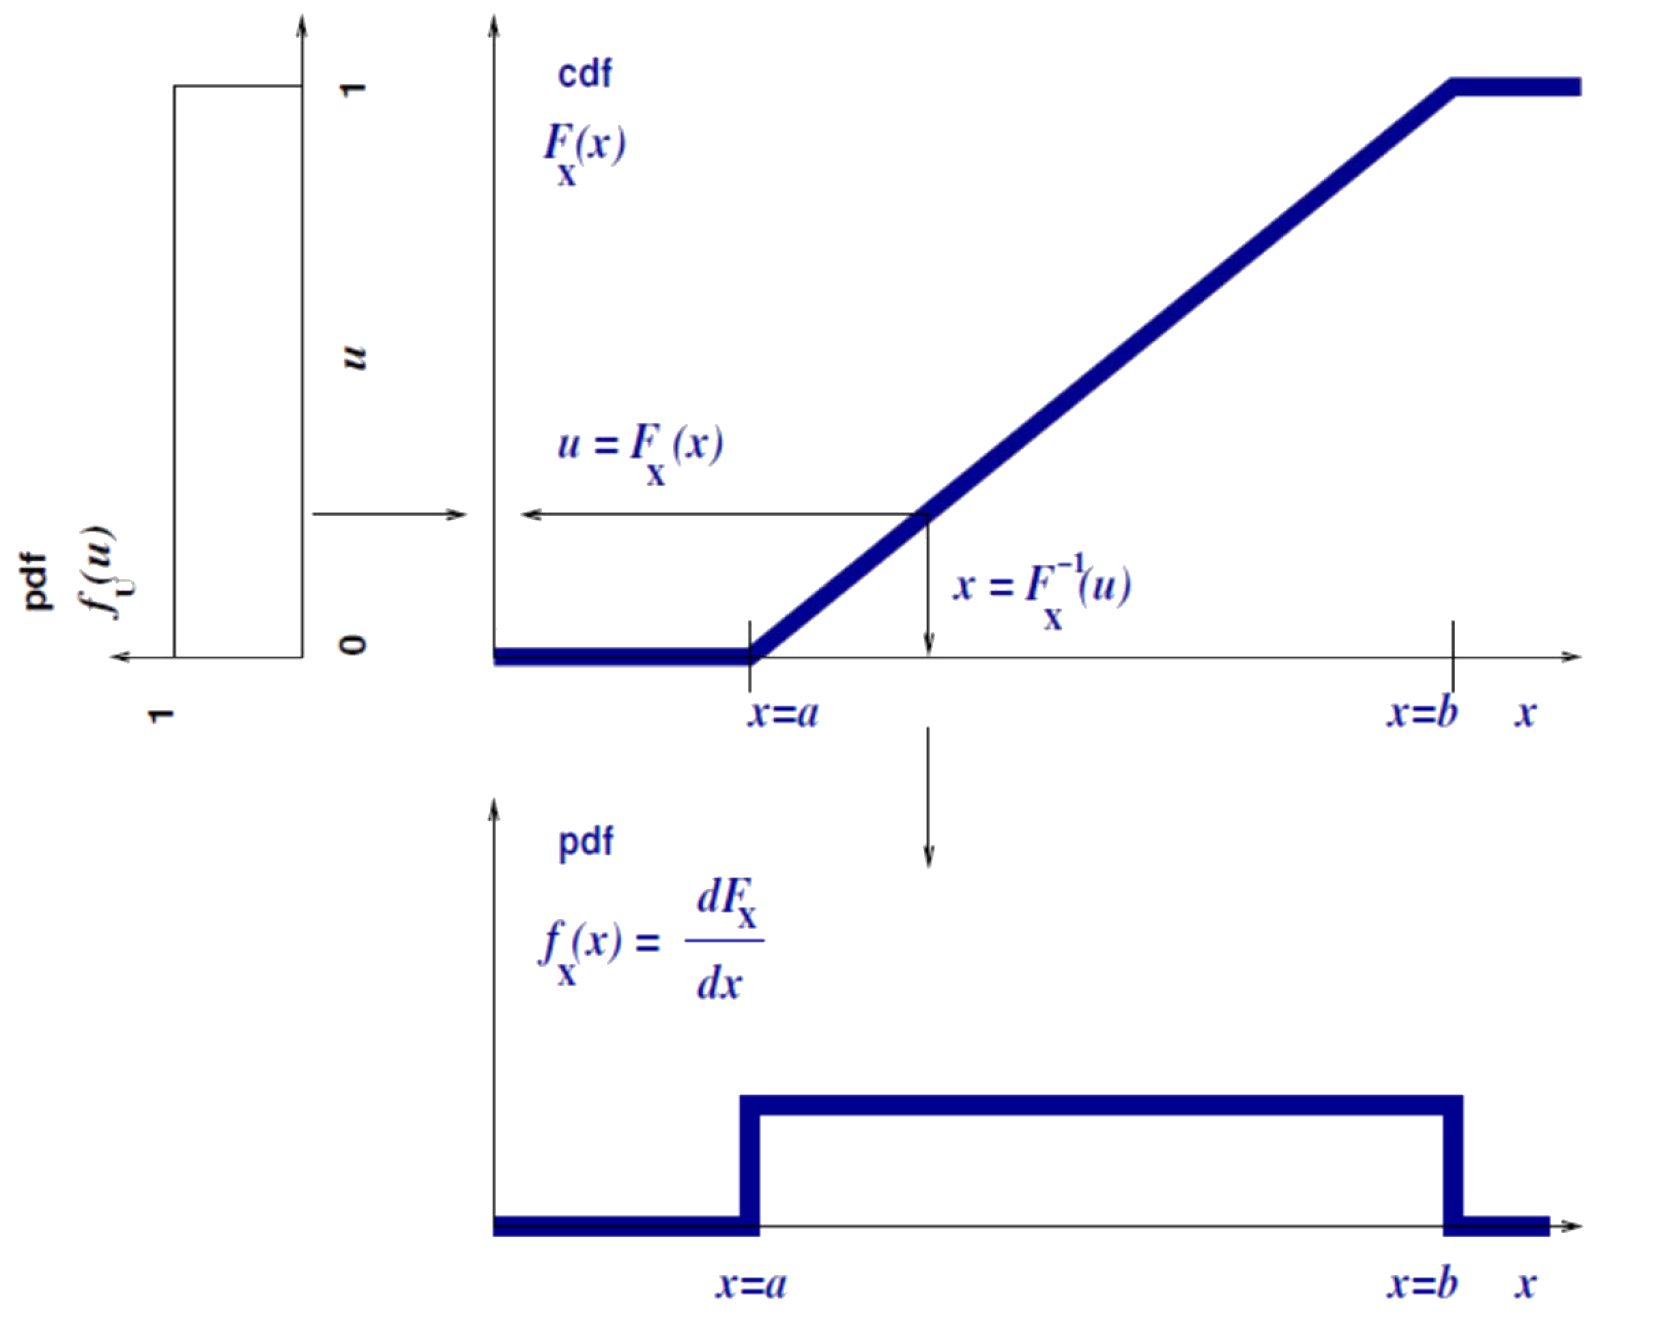
\includegraphics[width=0.33\textwidth]{pictures/inversionsmethode} 
	\end{multicols}
\end{example}

\begin{multicols}{2}
	\begin{example} 
		Exponentionalverteilung mit Parameter $\lambda$ \\
		\begin{compactitem}
			\item Gegeben: $x\sim U(0, 1)$
			\item Gesucht: $y\sim \exp (\lambda)$
			\item Beachte: $\begin{array}{l}
								F_y(y) = 1-e^{-\lambda y} \\
								x = 1-e^{-\lambda y} \\
								e^{-\lambda y} = 1-x\\
								y = -\frac{1}{\lambda}\ln (1-x)
							\end{array}$
		\end{compactitem}
	\end{example}
	\begin{example} 
		Empirische Verteilung \\
		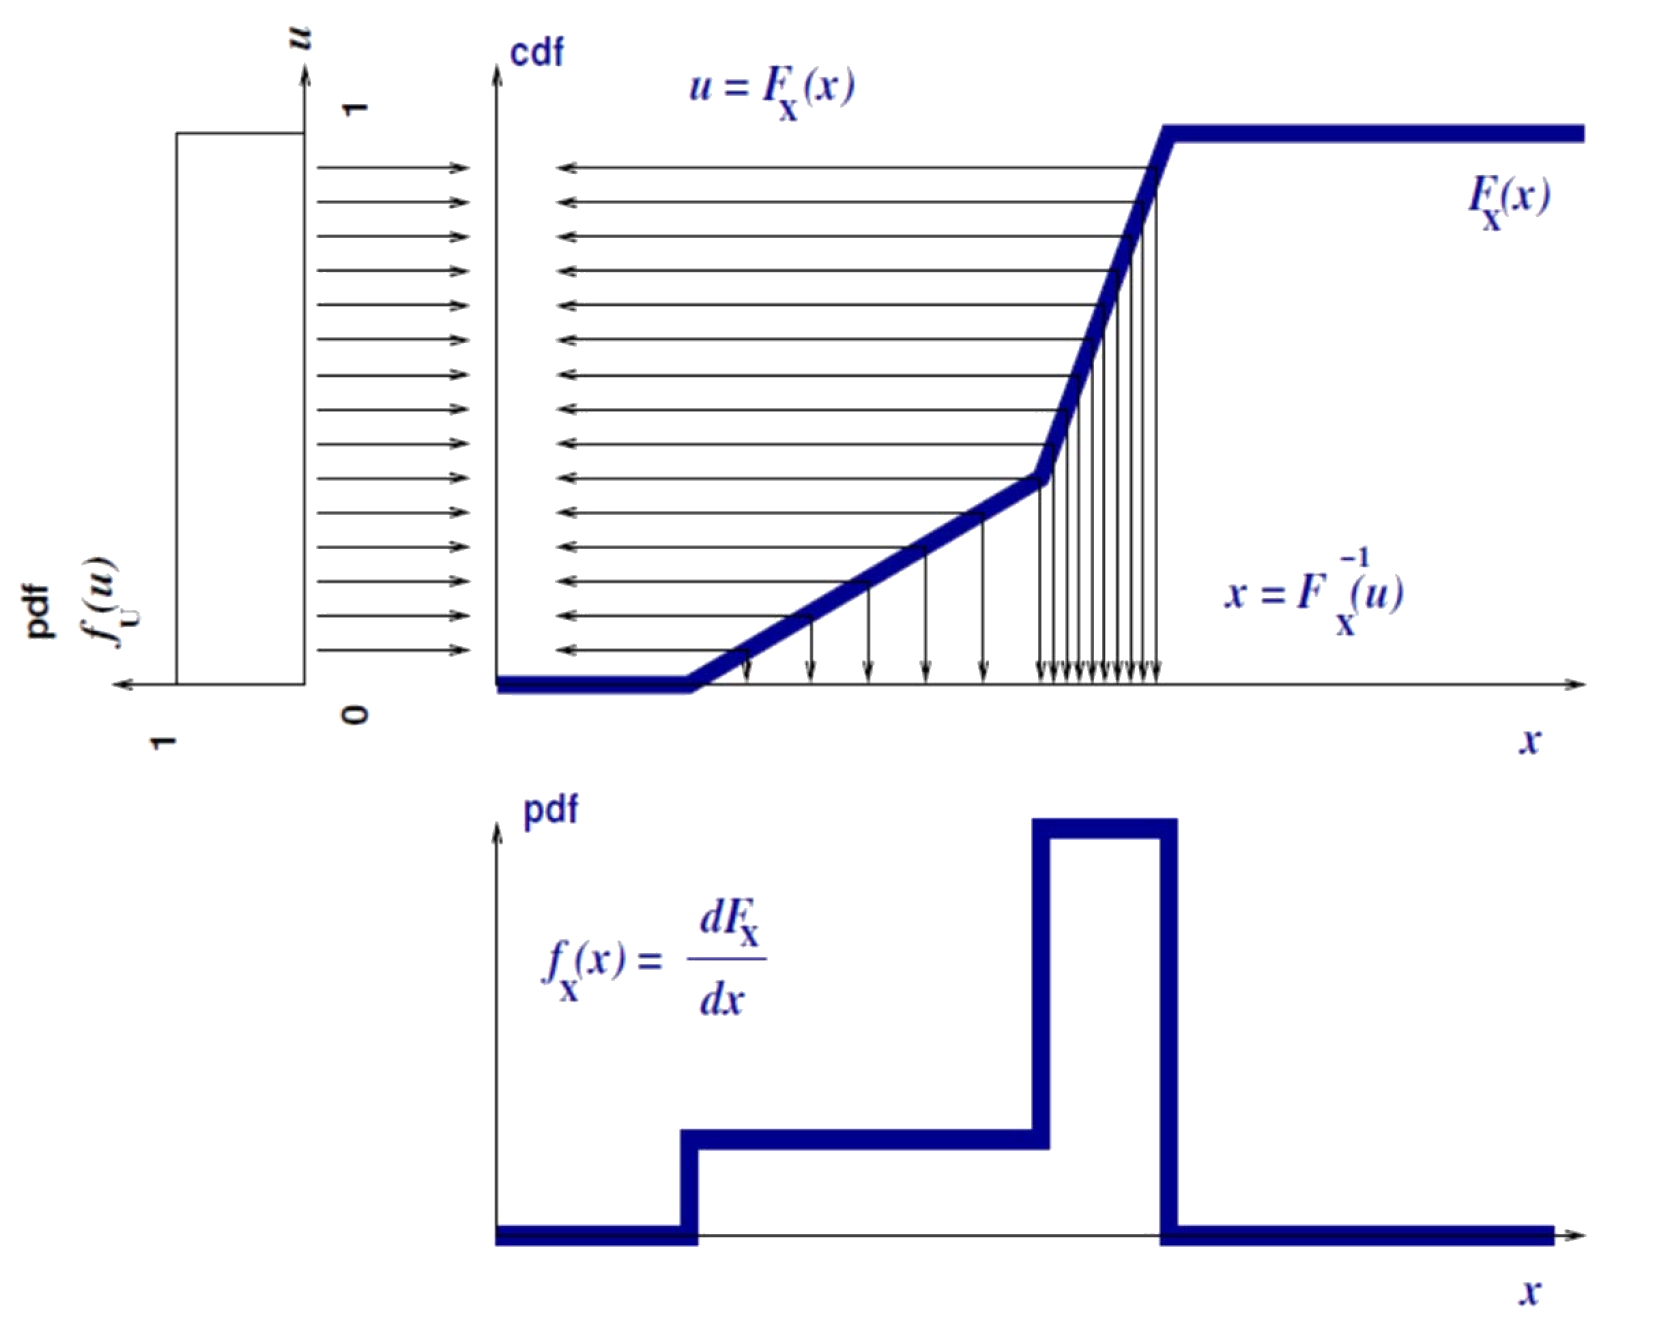
\includegraphics[width=1\textwidth]{pictures/inversionsmethode2} 
	\end{example}
\end{multicols}

\subsubsection{Wahl geeigneter Seedwerte}
\begin{compactitem}
	\item Der konkrete Seedwert spielt absolut keine Rolle (1, 2 oder 25343).
	\item Wichtig ist, ob Seedwerte identisch oder nicht-identisch sein sollten.
	\item Innerhalb eines Simulationslaufs: UNTERSCHIEDLICH
	\item Wenn wir 2 verschiedene Szenarien vergleichen wollen, wählen wir allerdings mit Vorteil Seed-Sätze, die identisch sind, um somit den \aszeichen{Zufallseinfluss} so weit wie möglich zu minimieren.
\end{compactitem}

\subsection{Ergebnisanalyse}
Simulationsergebnisse (z.B. durchschnittliche Wartezeiten in einer Arztpraxis) sind abhängig von Zufallszahlen (z.B. Behandlungsdauer, Zwischenankunftszeiten, usw.). Jedes Simulationsexperiment erzeugt neue Ergebnisse (solange Seed-Werte nicht fixiert sind). Simulationsergebnisse sind somit selbst auch Zufallszahlen!

\subsubsection{Konfidenzintervall}
Ein Konfidenzintervall (auch Vertrauensbereich oder Vertrauensintervall) ist ein Intervall aus der Statistik, das die Präzision der Lageschätzung eines Parameters (zum Beispiel eines Mittelwertes) angibt. Das Konfidenzintervall ist der Bereich, der bei unendlicher Wiederholung eines Zufallsexperiments mit einer gewissen Häufigkeit (dem Konfidenzniveau) die wahre Lage des Parameters einschliesst.
\begin{example}
	Die Anzahl Wanderer zwischen 9 und 10 Uhr morgens an der Talstation der Säntisbahn an einem sonnigen Tag in den Sommerferien bewegt sich mit einer Wahrscheinlichkeit von 95\% zwischen 50 und 200.\\
	Mathematisch: $P(X \in [50,200]) =  0.95$
\end{example}

\subsubsection{Batch-Mittelwert-Methode}
\begin{compactenum}
	\item Nach Einschwingverhalten, Gesamtzeit (resp. Gesamtmenge von Beobachtungen) in $n$ gleiche Batches teilen
	\item Mittelwert pro Batch berechnen
	\item Einzelmittelwerte mitteln (sofern Batches unabhängig voneinander sind, ist bei genügend langen Batches der Fall)
	\item Aus Streuung der Einzelmittelwerte Vertrauensintervall für Mittelwertschätzer bestimmen
\end{compactenum}
\begin{minipage}[h]{0.8\textwidth}
	\textbf{Mittelwert pro Batch:} $\hat{\theta}_i$\\
	\textbf{Einzelmittelwert:} $\hat{\theta}_n=\frac{1}{n}\sum_{i=1}^{n}\hat{\theta}_i$\\
	\textbf{Streuung:} $S_n^2=\frac{1}{n-1}\sum_{i=1}^{n}(\hat{\theta}_i-\hat{\theta}_n)^2$ \\
	\textbf{Konfidenzintervall:} $\hat{\theta}_n-z_{\frac{\alpha}{2}}\sqrt{\frac{\sigma^2}{n}} < \theta < \hat{\theta}_n+z_{\frac{\alpha}{2}}\sqrt{\frac{\sigma^2}{n}}$ mit $n$ = Anzahl Batches \\
	\textbf{Interpretation für n $>$ 29:} $P(\theta \in [\hat{\theta}_n-z_{\frac{\alpha}{2}}\sqrt{\frac{\sigma^2}{n}}, \hat{\theta}_n+z_{\frac{\alpha}{2}}\sqrt{\frac{\sigma^2}{n}}])=1-\alpha$
\end{minipage}
\begin{minipage}[h]{0.2\textwidth}
	\begin{tabular}{|l|l|}
		\hline
		$\alpha$ & $z_{\frac{\alpha}{2}}$ \\ \hline
		0.1 & 1.645 \\ \hline
		0.05 & 1.96 \\ \hline
		0.01 & 2.576 \\ \hline
	\end{tabular}
\end{minipage}	

\subsection{Reparierbare Systeme FCFS}
\subsubsection{Systembeschreibung} 
Wir betrachten komplexe technische Systeme wie z.B. Atomkraftwerke, Bohrinseln, Flugzeuge, Raketen oder Seebagger. Solche Systeme werden aus vielen kritischen, oft sehr teuren Bauteilen zusammengesetzt. Da System Stillstände enorme Kosten verursachen, müssen kritische Komponenten bei einem Ausfall möglichst schnell ausgetauscht werden können. Das ist nur möglich mit Hilfe von Lagerhaltung. Wenn eine kritische Komponente ausfällt, fliegt ein Hubschrauber mit einem funktionsfähigen Teil aus dem Lager zur Bohrinsel und bringt das defekte Teil zur Reparatur in eine Werkstatt auf dem Festland. 

\subsubsection{Annahmen}
\begin{compactitem}
	\item Jeder Komponente Ausfall führt zum Ausfall des gesamten Systems
	\item Ersatzteile und Systeme werden in einer einzigen Charge hergestellt
	\item Fehlerhafte Teile können immer repariert werden (und funktionieren anschliessend wieder wie neu)
	\item Es können nicht mehrere Teile gleichzeitig repariert werden! Dies bedeutet dass die Reparaturwerkstatt als Warteschlangensystem mit einem einzigen Schalter modelliert werden kann.
	\item Transportzeiten (Bohrinsel, Lager, Werkstatt) sind vernachlässigbar
\end{compactitem}

\subsubsection{Lösungsweg}
\begin{compactenum}
	\item Entwickle ein Simulationsmodell, das für einen gegebenen Stückzahlenvektor und eine gegebene Priorisierungsregel die durchschnittlichen jährlichen Gesamtkosten sowie den zeitlichen	Verlauf der Lagerbestände ermittelt.
	\item Entwickle durch Experimentieren mit dem Simulator eine geeignete Priorisierungsregel für die Reparaturwerkstatt.
	\item Entwickle ein simulationsbasiertes Optimierungsverfahren nach	folgendem iterativen Konzept. \\
	\begin{tikzpicture}[node distance = 0.6cm and 0.5cm]
		\node (middle) [answerW] {};		
		\node (optimierer) [decisionW, above=of middle] {Optimierer};
		\node (simulator) [decisionW, below=of middle] {Simulator};
		\node (lef) [decisionW, left=of middle] {Stückzahlenvektor, Priorisierungsregel Reparaturen};
		\node (rig) [decisionW, right=of middle] {Gesamtkosten, Zeitlicher Verlauf aller Lagerbestände};
		\draw [arrow] (optimierer) -| (lef);
		\draw [arrow] (lef) |- (simulator);
		\draw [arrow] (simulator) -| (rig);
		\draw [arrow] (rig) |- (optimierer);
	\end{tikzpicture}
\end{compactenum}

\subsubsection{Wahrscheinlichkeit} $f_i(k)$: die Wahrscheinlichkeit (gemessen als relativer Zeitanteil), dass die Anzahl kaputter Teile von Ersatzteil $i$ gleich $k$ ($k \geq 0$) ist.
\begin{example}
	Bestimme für die Simulation $f_i(k)$ \\
	\begin{minipage}[h]{0.7\textwidth}
		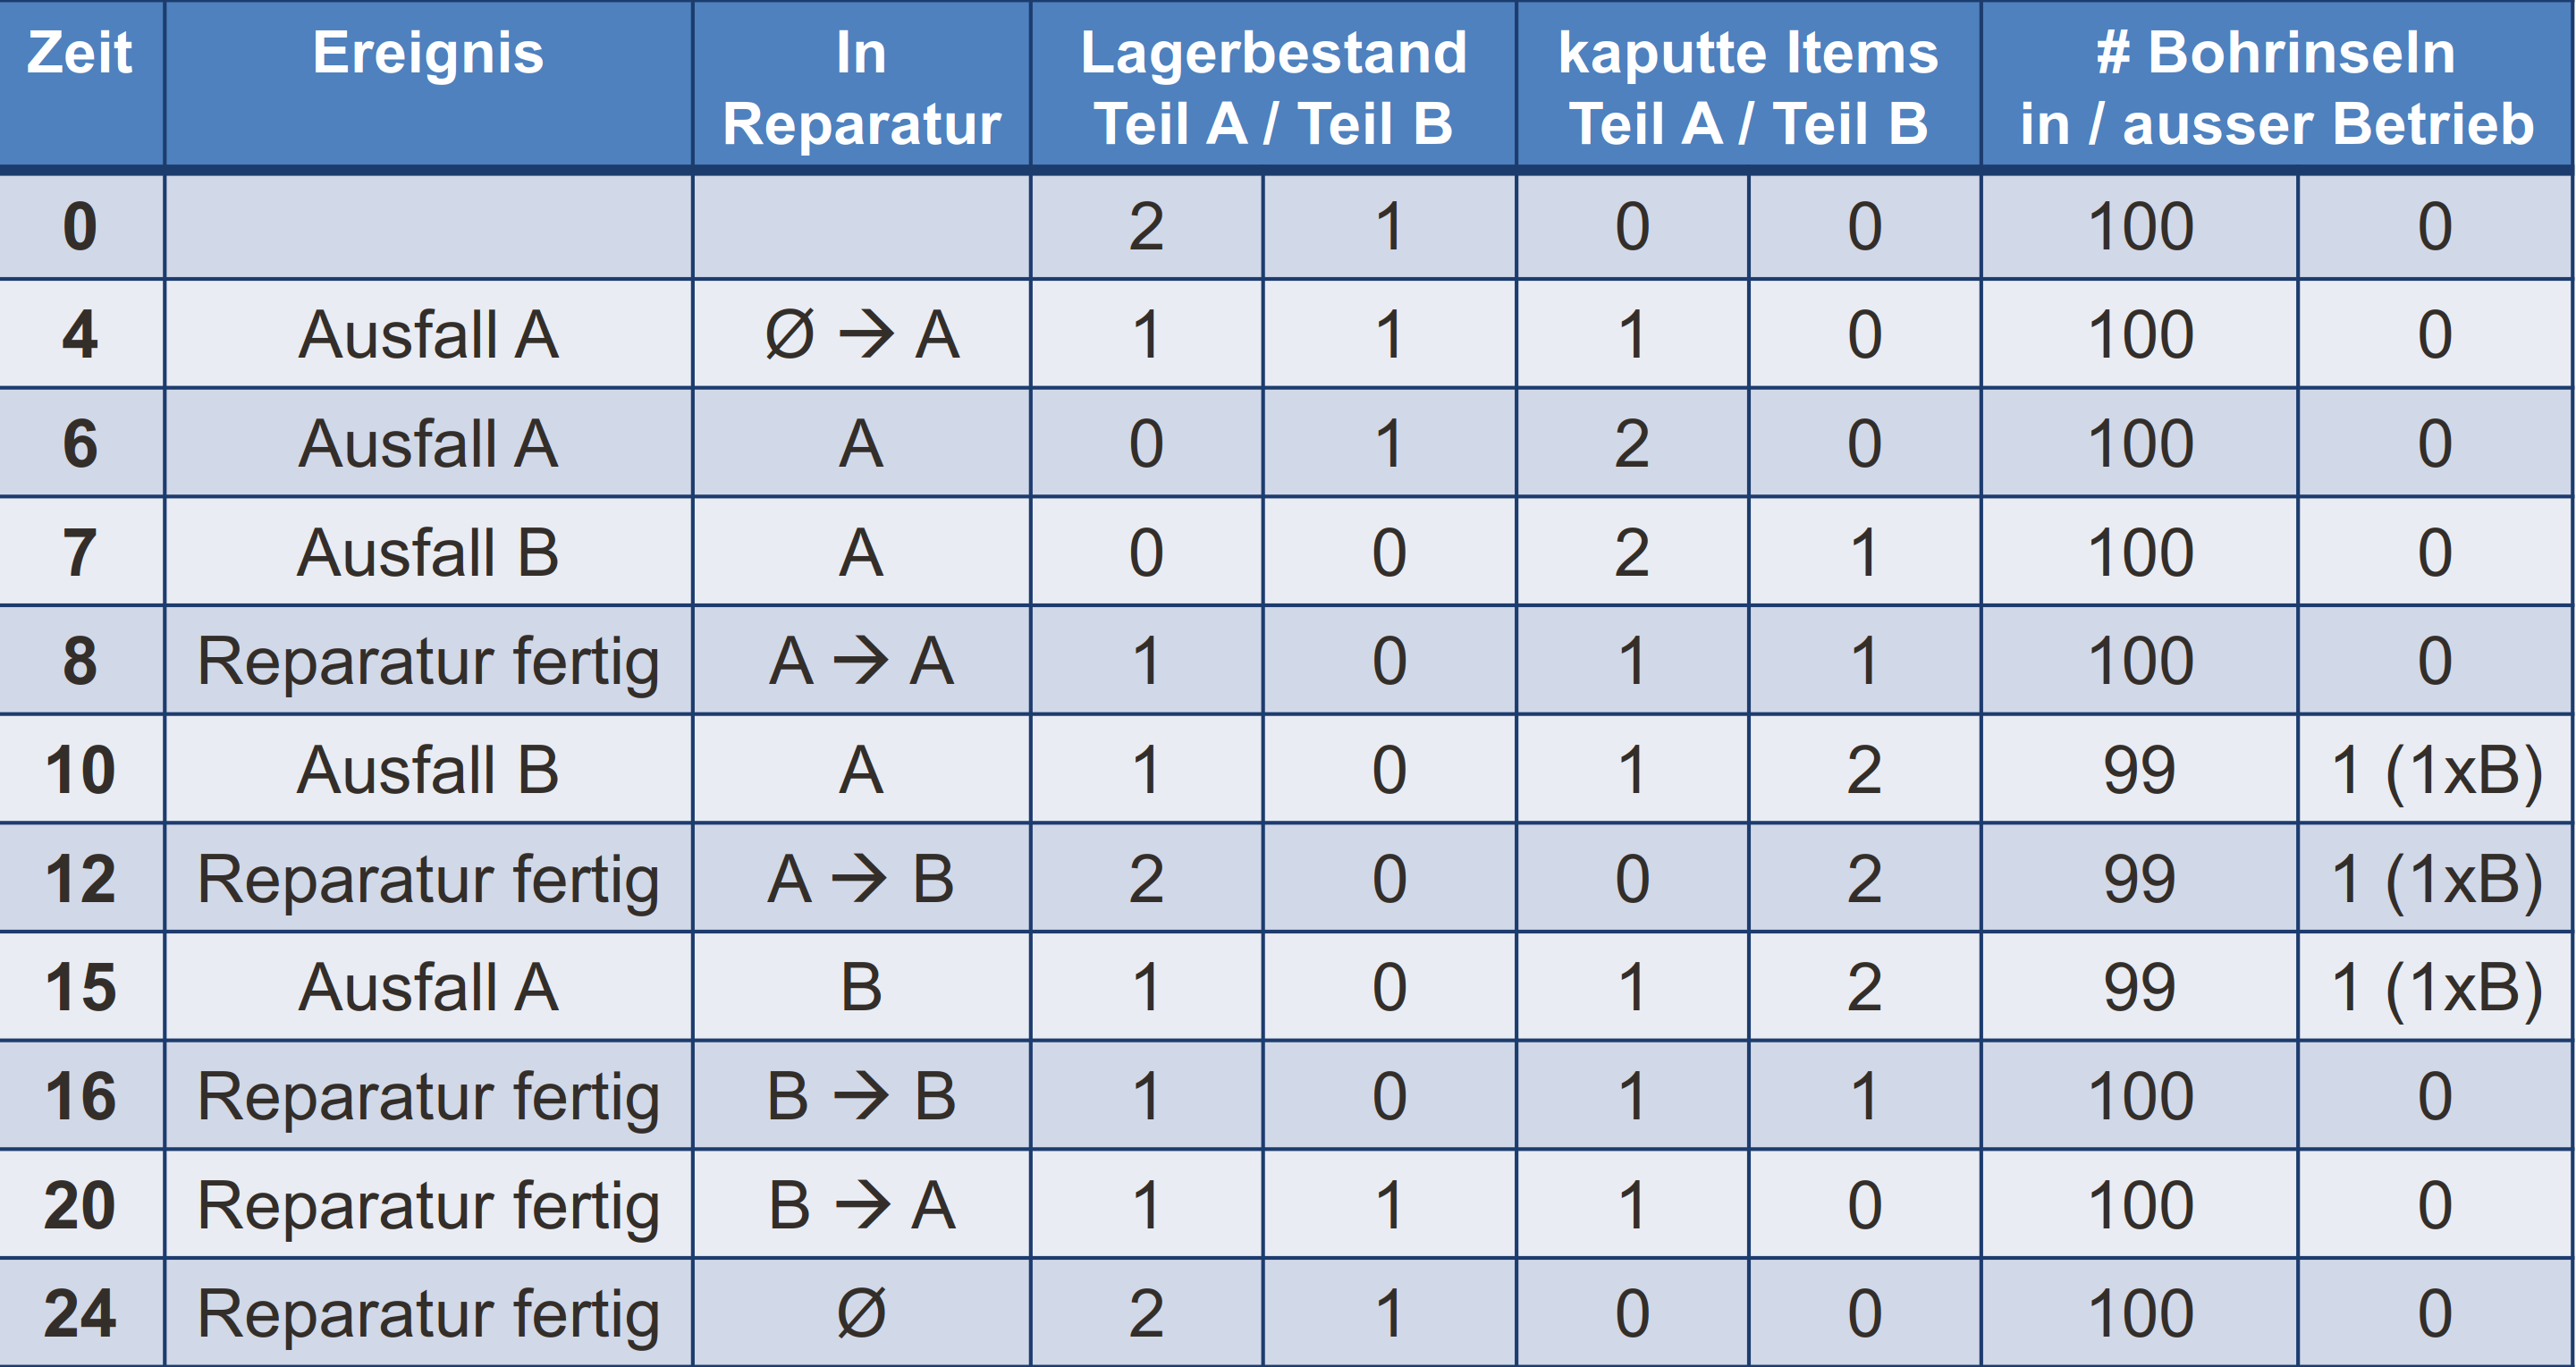
\includegraphics[width=0.95\textwidth]{pictures/reparatur} 
	\end{minipage}
	\begin{minipage}[h]{0.15\textwidth}
		\begin{tabular}{|l|l|}
			\hline
			k & $f_A(k)$ \\ \hline
			0 & 7/24 \\ \hline
			1 & 15/24 \\ \hline
			2 & 2/24 \\ \hline
			3 & 0 \\ \hline
		\end{tabular}
		\begin{tabular}{|l|l|}
			\hline
			k & $f_B(k)$ \\ \hline
			0 & 11/24 \\ \hline
			1 & 7/24 \\ \hline
			2 & 8/24 \\ \hline
			3 & 0 \\ \hline
		\end{tabular}
	\end{minipage}
\end{example}

\subsubsection{Auswirkungen Stückzahlenerhöhung} Pro Jahr werden CHF $[1-F(s)]b$ Stillstandskosten eingespart aber zusätzliche Ammortions- und Lagerkosten von CHF $c_i$ entstehen. Die Stückzahl wird solange erhöht, bis die marginalen Einsparungen $[1-F(s)]b$ die marginalen Kosten $c_i$ übertreffen.

\subsubsection{Strategie zur Bestimmung von optimalen Stückzahlen}
\begin{compactenum}
	\item Simuliere das System 1 x mit einem willkürlichen Stückzahlenvektor (z.B. 0) durch um $f_i(k)$ und somit $F_i(k)$ (i = 1, ..., N; k = 0, 1, ...) zu bestimmen.
	\item Für jeden Bauteil folgt anschliessend die optimale Stückzahl $S_i^*$ aus:	$S_i^* = \min \{Q|F_i(Q) \geq\frac{b-c_i}{b}\}$
\end{compactenum}

\subsubsection{Dynamische Priorisierung - Vorschlag}
\begin{compactenum}
	\item Bauteile die aktuell Stillstandskosten verursachen, werden priorisiert über solche die aktuell keine Stillstandskosten verursachen.
	\item Wenn mehrere Bauteile Stillstandskosten verursachen, wird das Bauteil mit der niedrigsten durchschnittlichen Reparaturzeit priorisiert über alle andere Bauteile.
	\item Wenn keiner der Bauteile aktuell Stillstandskosten verursacht, wird das Bauteil mit den kleinsten \aszeichen{Abdeckung} priorisiert, wobei \aszeichen{Abdeckung} definiert wird als (aktueller Lagerbestand + 1) x durchschnittliche Zeit zwischen zwei nachfolgenden Ausfällen
\end{compactenum}
\textbf{Beschriebene Strategie zur Optimierung der Stückzahlen unter FCFS kann nicht 1 : 1 verwendet werden.}

\subsubsection{Simulationsbasierte Optimierung (iterativ)}
\begin{compactenum}
	\item Entwerfe intelligente Priorisierungsregel $\Omega$
	\item Setze Iterationszahl $n = 0$ und initialisiere $S^n = 0$
	\item  Simuliere das System unter Verwendung von $\Omega$ und $S^n$. Speichere die relativen Häufigkeiten der defekten Teile $i$, $f_i(k)$, $k \geq 0$.
	\item Berechne $S^{n+1} = \min \{Q|F_i(Q) \geq\frac{b-c_i}{b}\}$
	\item Beende die Iteration, wenn $S^{n+1} = S^n$. Andernfalls setze $n = n + 1$ und gehe zu Schritt 3.
\end{compactenum}
\end{document}